% =============================================================================
% Membrane Cosmology v4.8 companion paper
%   FIRAS mu-distortion upper bound and universal density coupling
%   closed-form derivation (foundation layer)
%
%   Sakaguchi Shinobu (坂口 忍), 2026-04
%   Migrated from ReportLab PDF (v3 patched, 13 pages)
%   Target: arXiv astro-ph.CO + hep-th cross
%
%   Compile: lualatex membrane_v48 && bibtex membrane_v48 && lualatex x2
% =============================================================================
\documentclass[11pt,a4paper]{ltjsarticle}

% ---------------- core packages ---------------------------------------------
\usepackage[a4paper,margin=20mm,headheight=14pt]{geometry}
\usepackage{amsmath,amssymb,amsthm}
\usepackage{mathtools}
\usepackage{booktabs}
\usepackage{array}
\usepackage{tabularx}
\usepackage{longtable}
\usepackage{graphicx}
\graphicspath{{figures/}}
\usepackage{xcolor}
\usepackage{titlesec}
\usepackage{enumitem}
\usepackage{fancyhdr}
\usepackage[hidelinks,breaklinks=true]{hyperref}
\usepackage[round,authoryear,sort&compress]{natbib}
\usepackage[most]{tcolorbox}

% ---------------- Japanese font setup (luatexja) ----------------------------
\usepackage[no-math]{luatexja-fontspec}
\setmainjfont[BoldFont=IPAGothic]{IPAPGothic}
\setsansjfont{IPAGothic}

% ---------------- section formatting ----------------------------------------
\titleformat{\section}{\normalfont\Large\bfseries}{\thesection}{0.6em}{}
\titleformat{\subsection}{\normalfont\large\bfseries}{\thesubsection}{0.6em}{}
\titleformat{\subsubsection}{\normalfont\normalsize\bfseries}{\thesubsubsection}{0.6em}{}
\titlespacing*{\section}{0pt}{3.2ex plus 1ex minus .2ex}{1.6ex plus .2ex}
\titlespacing*{\subsection}{0pt}{2.4ex plus .8ex minus .2ex}{1.2ex plus .2ex}

% ---------------- colors (boxed notes) --------------------------------------
\definecolor{colKey}{RGB}{230,242,252}   % key finding (pale blue)
\definecolor{colNote}{RGB}{240,246,252}  % note (very pale blue)
\definecolor{colWarn}{RGB}{255,243,220}  % warning (pale orange)
\definecolor{colMath}{RGB}{245,245,250}  % math background (pale gray)

% ---------------- boxed environments (tcolorbox-based) ---------------------
\newtcolorbox{keybox}{
  enhanced, breakable, colback=colKey, colframe=colKey!80!black,
  boxrule=0.3pt, arc=1pt, left=6pt, right=6pt, top=4pt, bottom=4pt,
  before skip=6pt, after skip=6pt
}
\newtcolorbox{notebox}{
  enhanced, breakable, colback=colNote, colframe=colNote!80!black,
  boxrule=0.3pt, arc=1pt, left=6pt, right=6pt, top=4pt, bottom=4pt,
  before skip=6pt, after skip=6pt
}
\newtcolorbox{warnbox}{
  enhanced, breakable, colback=colWarn, colframe=colWarn!80!black,
  boxrule=0.3pt, arc=1pt, left=6pt, right=6pt, top=4pt, bottom=4pt,
  before skip=6pt, after skip=6pt
}

% ---------------- number formatting macros ----------------------------------
% \Ten{-53} -> \times 10^{-53}
\newcommand{\Ten}[1]{\times 10^{#1}}
% \ee{2.96}{-53} -> 2.96 x 10^{-53}  (exponent-form number)
\newcommand{\ee}[2]{#1 \times 10^{#2}}

% ---------------- physics symbol shortcuts ----------------------------------
\newcommand{\epso}{\epsilon_0}
\newcommand{\kmem}{k_{\mathrm{mem}}}
\newcommand{\cmem}{c_{\mathrm{mem}}}
\newcommand{\Vxi}{V_{\xi}}
\newcommand{\Vxivoid}{V_{\xi,\mathrm{void}}}
\newcommand{\Tm}{T_{m}}
\newcommand{\Nmode}{N_{\mathrm{mode}}}
\newcommand{\nmode}{n_{\mathrm{mode}}}
\newcommand{\aPT}{\alpha_{\mathrm{PT}}}
\newcommand{\taum}{\tau_{m}}
\newcommand{\taur}{\tau_{\mathrm{relax}}}
\newcommand{\bal}{b_{\alpha}}
\newcommand{\umem}{u_{\mathrm{mem}}}
\newcommand{\rhomem}{\rho_{\mathrm{mem},0}}
\newcommand{\rhog}{\rho_{\gamma,0}}
\newcommand{\rhogal}{\rho_{\mathrm{gal}}}
\newcommand{\Imu}{I_{\mu}}
\newcommand{\Wmu}{W_{\mu}}
\newcommand{\APT}{A_{\mathrm{PT}}}
\newcommand{\BFIRAS}{B_{\mathrm{FIRAS,combo}}}
\newcommand{\Lambdauv}{\Lambda_{\mathrm{UV}}}
\newcommand{\GammaA}{\Gamma_{A}}
\newcommand{\GammaAp}{\Gamma_{A}'}
\newcommand{\GammaB}{\Gamma_{B}}
\newcommand{\GammaC}{\Gamma_{C}}
\newcommand{\Gammaref}{\Gamma_{\mathrm{ref}}}
\newcommand{\Gammaact}{\Gamma_{\mathrm{actual}}}
\newcommand{\muFIRAS}{\mu_{\mathrm{FIRAS}}}
\newcommand{\ZMU}{Z_{\mu}}
\newcommand{\ZDC}{Z_{\mathrm{DC}}}
\newcommand{\msigma}{m_{\sigma}}
\newcommand{\gobs}{g_{\mathrm{obs}}}
\newcommand{\gbar}{g_{\mathrm{bar}}}
\newcommand{\gc}{g_{c}}
\newcommand{\vflat}{v_{\mathrm{flat}}}
\newcommand{\hR}{h_{R}}
\newcommand{\Yd}{\Upsilon_{d}}
\newcommand{\Jhalf}{J_{\mathrm{half}}}
\newcommand{\clt}{c_{\mathrm{lt}}}       % light-time speed (c)
\newcommand{\fopt}{f_{\mathrm{opt}}}
\newcommand{\Rvoid}{R_{\mathrm{void}}}
\newcommand{\vchar}{v_{\mathrm{char}}}
\newcommand{\AIC}{\Delta\mathrm{AIC}}
\newcommand{\LOO}{\mathrm{LOO}}

% ---------------- title data ------------------------------------------------
\title{\bfseries 膜宇宙論 foundation layer:\\
FIRAS $\mu$ 歪み上限と universal density coupling の閉形式導出\\[2pt]
\large --- v4.7.8 companion paper (v4.8) ---}
\author{坂口 忍 (Sakaguchi Shinobu)\\
\small 坂口製麺所(兵庫県宍粟市)~/~\texttt{sakaguchi-physics.com}}
\date{2026 年 4 月版}

% =============================================================================
\begin{document}
\maketitle
\thispagestyle{empty}

% ---------------- Abstract --------------------------------------------------
\begin{abstract}
\small\noindent
膜宇宙論 v4.7.8 本体~\citep{Sakaguchi2026a} は SPARC 175 銀河、dSph 31 銀河、HSC-SSP Y3 + GAMA DR4 + KiDS
の独立 3 field で Condition 15 (C15) を A 級 establish し、MOND を
$p = 1.66 \times 10^{-53}$ で棄却した。本 companion paper はその observational establishment
を支える理論的 foundation layer を閉形式で与え、観測との整合性を NGC 3198 anchor で 2.32\% 一致として確認する。

\smallskip\noindent
核心的成果は 5 点:
(M1) FIRAS $\mu$ 歪み~\citep{Fixsen1996} を Chluba 2016 $\Wmu$ kernel で展開し、$\Vxi$ primary 採用で
$\aPT^{\mathrm{upper}}$ (phase transition coupling 上限) を 3 銀河 anchor (IC 2574 / NGC 3198 / NGC 2841)
per-galaxy 評価として導出。代表値は $\aPT^{\mathrm{upper}}(\mathrm{NGC\,3198}, \Vxi) = 1.76 \times 10^{-51}$
(MRT 統一 anchor, v4.8 v1 版の $2.96 \times 10^{-53}$ は v37 convention 由来の 2-pt 外挿 artifact で factor 59 弱い; \S 7.3 参照)。
3 銀河 range は $[1.6 \times 10^{-53},\, 1.8 \times 10^{-50}]$ (≈3 桁幅)。
(M2) $\aPT^{\mathrm{upper}}$ を通じて membrane memory time $\taum$ に
$[1.9 \times 10^{10},\; 1.4 \times 10^{53}]$ s の FIRAS-only bound を与え、Local Void ($R=22$ Mpc)
の因果律制約で 5 桁幅に narrow 化 (38 桁 tighten)。
(M3) mode 数 $\Nmode$ の SI canonical 定義 (Eq. 2B-II) により、NGC 3198 の
$\kmem \cdot \Nmode$ product が 2.32\% 精度で再現 (A 級)。
(M4) 記号 $\chi$ が担う 2 変数 $\chi_E\,[\mathrm{s}^2]$ と $\chi_F\,[\mathrm{m}^{3/2}/\mathrm{s}^2]$
は独立であり、universal conversion は存在しないことを明示。
(M5) Pantheon+ \citep{Scolnic2022} による $f=0.379$ は $\mu$ kernel に寄与しない (explicit null)。

\smallskip\noindent
加えて SPARC 124 銀河 (bridge 除外後) と dSph 30 銀河で得た coupling slope
$\bal = +0.1084$ vs $+0.1127$ は 3.92 dex の密度範囲で 0.5\% 以内に一致し、
$\umem \cdot \rhogal^{2\bal}$ の universal coupling を operational に establish する
(C3 内部メモ v3 A 級)。本結果は $\alpha$ (linear) vs $\gamma$ (threshold) のモデル弁別を
Akaike 情報量基準で $\alpha$ 優位 ($\AIC = -2.00$) に決着し、dark matter 粒子模型が必要としない
``variation efficiency $\sim 11\%$ (amplitude) / $\sim 5.5\%$ (power)'' という operational 制約を与える。
両数値は同一 $\bal=0.11$ に対する基準選択の差 ($\rho^1$ amplitude vs $\rho^2$ power) であり、
第一原理的変換効率は C3-3 ($\taum$ 物理見積) + \S 7.8 (C3-4 P1-P4 分岐比) 完了待ちの heuristic 併記である。

\smallskip\noindent
限界: (i) 無次元 $\Tm = \sqrt{6}$ の SI 絶対較正は foundation 内部では決定不能で、
$\sigma$ rest energy 候補と membrane coherence 候補の間に 96 桁 gap が残る。
(ii) membrane memory rate $\Gammaact$ の絶対値決定は 3 route (normal mode / FDT / 観測 proxy) の
並行評価に留まり、$\taur$ 物理選択を要する energy branching 問題に帰着する。
これら限界は v4.8 次版 (21cm + CMB TT cross-check) で対処予定。

\smallskip\noindent\textbf{Keywords:} membrane cosmology, dark matter alternative, MOND rejection,
FIRAS $\mu$-distortion, universal density coupling, C15
\end{abstract}

\clearpage

% =============================================================================
\section{Introduction}
% =============================================================================

\subsection{Observational establishment (v4.7.8 本体)}
膜宇宙論 v4.7.8 本体~\citep{Sakaguchi2026a} は dark matter 現象を粒子ではなく
膜折れ畳み構造由来とする framework で、観測的に以下を establish した:
(i) Condition 15 最終形 $\gc = 0.584 \cdot \Yd^{-0.361} \cdot \sqrt{a_0 \cdot \vflat^2 / \hR}$ を
SPARC 175 銀河で $R^2 = 0.607$、$\AIC = -14.2$、LOO-CV 安定で確立~\citep{Lelli2016c}。
(ii) Bernoulli 普遍関係 $G_{\mathrm{Strigari}} = s_0 (1 - s_0)\,a_0 = 0.228\,a_0$ を dSph 31 銀河
($0.240\,a_0$、4\% 以内) と SPARC bridge 外側 30 点 ($0.219\,a_0$、4\% 以内) の 2 独立サンプルで
再現~\citep{McConnachie2012, Strigari2008}。
(iii) HSC-SSP Y3 + GAMA DR4 の 3 field 統合 (157{,}338 lenses, 503M pairs) で
$\gc = 2.73 \pm 0.11\,a_0$ 独立再現、$\AIC(\mathrm{C15\;vs\;MOND}) = +472$ (22 $\sigma$)。
(iv) MOND を $p = 1.66 \times 10^{-53}$ で棄却。

\subsection{なぜ companion paper が必要か}
v4.7.8 は現象論的には完結している (19 結論)。しかし各 condition の物理的由来
(何故 $\gc$ がこの関数形なのか、$\taum$ はどの範囲にあるのか、$\aPT$ は何を意味するのか) は
本体では簡潔に触れるに留まった。本 companion paper は v4.7.8 の結論を変えずに、
その theoretical foundation を 11 以上の閉形式の連鎖として明示する。

本構造は single-paper で扱うには材料が過剰 (v4.7.8 既に 12 頁) であり、分離 publish
の方が観測派読者と理論派読者の双方に accessible と判断した (Session +6 確定の分離戦略)。
本 companion paper は v4.8 として arXiv に独立投稿し、v4.7.8 とは非干渉に成立する。

\subsection{本論文の構成 (roadmap)}
\S 2 で Q-core 3 判断と Form B ポテンシャルを導入し、膜 strain field $\epsilon$ の
平衡分散を与える Fluctuation-Dissipation 関係 (Eq. I) を出発点として
4 主式 (Eq. I, II-b, II-d, III, IV) を連鎖接続する (foundation\_$\alpha$1)。
\S 3 で mode 数 $\Nmode$ の SI canonical 定義 (Eq. 2B-II) と UV cutoff $\Lambdauv$ の symbolic
閉形式 (Eq. 2C-0) を与える (foundation\_$\alpha$2)。
\S 4 で FIRAS $\mu$ 歪みを Chluba 2016 $\Wmu$ kernel で展開し、
$\aPT^{\mathrm{upper}}$ と $\taum$ bound を導出。
\S 5 で観測との cross-check (NGC 3198 2.32\% PASS、universal $\bal = 0.11$ across 3.92 dex) を提示。
\S 6 で 5 main claims M1--M5 を整理、\S 7 で限界と将来課題を論じる。
Appendix に全数値 anchor と参考文献を収録。

\begin{notebox}
\textbf{読者への注意:}
本論文は閉形式の連鎖
(Eq. I $\to$ II-b $\to$ II-d $\to$ III $\to$ IV $\to$ 2A-I/II $\to$ 2B-I/II $\to$ 2C-0 $\to$
iv-d-I/II/III/IV $\to$ iv-e-I)
を追うことを主目的とし、個々の導出詳細は付属成果物
\texttt{foundation\_integrated.pdf} (15 頁、Appendix A で cross-reference) に委ねる。
本論文は argument 構造の明示に集中するため、計算の再現は付属 script
(\texttt{uv run} で実行可能、Windows Claude Code 環境確認済) で担保する。
\end{notebox}

\subsection{Main claims (M1--M5) の予告}
\begin{center}\small
\begin{tabular}{@{}c>{\raggedright\arraybackslash}p{75mm}l>{\raggedright\arraybackslash}p{45mm}@{}}
\toprule
\# & Claim & 節 & 核心数値 \\
\midrule
M1 & $\aPT^{\mathrm{upper}}(\mathrm{NGC\,3198},\Vxi) = 1.76 \times 10^{-51}$ (anchor), 3-gal range $[1.6\times10^{-53},\,1.8\times10^{-50}]$ & \S 4 & FIRAS $\mu < 9 \times 10^{-5}$ \\
M2 & $\taum$ bound $[1.9 \times 10^{10},\, 1.4 \times 10^{53}]$ s $\to$ 5 桁幅 & \S 4, 5 & Local Void $R=22$ Mpc \\
M3 & Eq. 2B-II SI canonical & \S 3 & NGC 3198 2.32\% PASS \\
M4 & $\chi_E,\chi_F$ 独立 (universal conversion 不存在) & \S 3, 7 & $[\mathrm{s}^2]$ vs $[\mathrm{m}^{3/2}/\mathrm{s}^2]$ \\
M5 & $f=0.379$ $\mu$ kernel 非寄与 (explicit null) & \S 7 & Pantheon+ \citep{Scolnic2022} \\
\bottomrule
\end{tabular}
\end{center}

% =============================================================================
\section{Theoretical Framework: Form B + FDT + Picture T}
% =============================================================================

\subsection{Q-core 3 判断}
全 foundation の起点として 3 判断を採用する。これらは内部整合性と観測 anchor の両方から
要請される minimal な選択で、以降の閉形式は全て 3 判断を前提とする。

\begin{keybox}
\textbf{Q-core1 (C-judge):} $\chi_E = a_0 / \kmem\;[\mathrm{s}^2]$\\
\quad MOND 外部 anchor $a_0$ 採用により循環参照を回避。\\[2pt]
\textbf{Q-core2 (P-T):} $\msigma^2$ (static curvature) と $\taum$ (dynamic relaxation) は
直交する独立 product として結合する。\\[2pt]
\textbf{Q-core3 (段階採用):} Stage 1 (volume avg) $\to$ Stage 2 (精密化) の 2 段。
\end{keybox}

\subsection{Form B ポテンシャルと $\Tm=\sqrt{6}$}
effective potential $U(\epsilon; c) = -\epsilon - \epsilon^2/2 - c\,\ln(1 - \epsilon)$ を採用
(Form B、v4.7.6 確立)。$dU/d\epsilon = 0$ から $\epso = \sqrt{1 - c}$ が得られ、
$w(c)^2 = U''(\epso) = 2\epso/(1 - \epso)$ が thermodynamic stability を
$c \in (0, 1)$ の全域で保証する。canonical $c_0 = 0.83$ (SPARC+dSph volume average) で
$\epso = 0.412311$、$w(c)^2 = 1.4032$。

$Z_2$ 対称性自発的破れの臨界温度 $\Tm = \sqrt{6}$ を無次元で与える (補題 5、v4.7.6 A 級)。
本値は 4-point correlator の Gaussian 評価と mean-field 臨界指数 $z \cdot \nu = 1/2$ の連立から
得られる universal constant。物理単位への翻訳 (ケルビン等価) は本 foundation 内部では
決定不能 (\S 7 参照)。

\subsection{foundation\_$\alpha$1: 4 主式}
膜 strain field の Langevin dynamics から、以下 4 主式が連鎖して得られる (Session +2--+6 で確立)。

\begin{keybox}
\begin{align*}
\text{Eq. I (FDT):}\quad &\langle \delta\epsilon^2 \rangle_{\mathrm{eq}} = \Tm / w(c)^2 = 1.745 \quad (c_0 = 0.83) \\
\text{Eq. II-b:}\quad &\msigma^2(c) = 4\epso \cdot w(c)^2 \cdot (\kmem / a_0) \\
\text{Eq. II-d:}\quad &\Jhalf(c) = (8\kmem^2 \Tm^2 \Gamma / a_0^2) \cdot \epso(1 - \epso) \\
\text{Eq. III:}\quad &\msigma^2 \cdot \langle \delta\epsilon^2 \rangle_{\mathrm{eq}} = 4\epso\Tm \cdot (\kmem / a_0) \\
\text{Eq. IV:}\quad &\mu = \APT \cdot \Imu \quad \text{(Stage 1/2 因数分解)}
\end{align*}
\end{keybox}

Eq. III は Eq. I と Eq. II-b の積から $w(c)^2$ が消去される構造的恒等式で、右辺は $c_0$ の関数として
$\epso$ のみに帰着する。Jeans volume-halved $\Jhalf$ は Phase C2 dSph 解析で Strigari 関係と独立に
30 銀河再現 ($\pm 5\%$)、閉形式の観測 anchor として機能する。

\medskip\noindent
\textbf{Eq. IV の因数分解:}
$\mu$ 歪み $= \APT$ (prefactor) $\cdot \Imu$ (kernel integral) の直積。
\[
\APT = \frac{4\aPT \Tm \kmem \Gamma \Nmode}{a_0} \cdot \frac{\rhomem^2}{\rhog}.
\]
$\Imu$ は Chluba $\Wmu$ kernel 下の integral で Stage 1 (closed form) と Stage 2 (精密) に分離される。
$\mathrm{S2/S1} = 0.8747$ が $c_0$ 非依存 ($\mathrm{std} = 2 \times 10^{-16}$、機械精度) であることが
\S 4 で示すように integrand 構造の正しさの強い証左となる。

% =============================================================================
\section{foundation\_$\alpha$2: $\cmem$ + $\Nmode$ + $\Lambdauv$}
% =============================================================================

\subsection{Step 2-A: 膜固有音速 $\cmem$ と $\chi_F$}
膜音速 $\cmem$ を Q-core1 の $\chi$ に接続する force-conjugate 量として $\chi_F$ を新たに定義する。
$\chi$ は記号上の同一性から混同を招きやすいが、次元で明瞭に区別される (後述 M4)。

\begin{keybox}
\begin{align*}
\text{Eq. 2A-I:}\quad &\kmem^2 = a_0 / \cmem^2 \\
\text{Eq. 2A-II:}\quad &\chi_F = \cmem \cdot \sqrt{a_0}\;\; [\mathrm{m}^{3/2}/\mathrm{s}^2]
\end{align*}
\end{keybox}

$\cmem$ の数値評価は v3.7 Chap 18 Table 18-3 の銀河別 $\fopt(c) \cdot \vflat$ mapping を用いる。
以下は 3 anchor 銀河 (IC 2574 / NGC 3198 / NGC 2841) の per-galaxy 値 (MRT 統一 $\vflat$, Lelli 2016):

\begin{center}\small
\begin{tabular}{@{}llllll@{}}
\toprule
Galaxy & $c$ & $\fopt(c)$ & $\vflat$ [m/s] & $\cmem$ [m/s] & $\chi_F$ [m$^{3/2}$/s$^2$] \\
\midrule
IC 2574  & 0.30 & 0.797 & $6.64 \times 10^{4}$ & $5.29 \times 10^{4}$ & 0.579 \\
NGC 3198 & 0.42 & 1.010 & $1.501 \times 10^{5}$ & $1.516 \times 10^{5}$ & 1.661 \\
NGC 2841 & 0.80 & 1.845 & $2.848 \times 10^{5}$ & $5.254 \times 10^{5}$ & 5.754 \\
\bottomrule
\end{tabular}
\end{center}

v4.8 v1 版で採用した $\fopt(0.83) = 1.9163$ は NGC 3198 ($c=0.42$, $\fopt=1.01$) と NGC 2841
($c=0.80$, $\fopt=1.85$) の 2 点 $\fopt$-linear 外挿 artifact であった (patch spec v2 \S 6.3 /
retract 不可 \#41)\footnote{$\epsilon_{\mathrm{scale}}$ パラメータの CMB-side operational
coupling (Plik TT likelihood に対する linear $(\epsilon_{\mathrm{scale}}-1)$
modification ansatz) は \S 5.5 Eq. 5.5-I + Eq. 5.5-II で Phase 5-2 chain
B-2 用に導入される。本 \S 3 の foundation\_$\alpha$2 では数値較正対象外
(operational ansatz の formal grounding は v4.9 patch round deferred、
\S 6.8)。}. 本 v3 erratum では v3.7 Chap 18-2 の 5 点
$c \in \{0.30, 0.42, 0.618, 0.80, 1.00\}$ から deg-4 exact-pass Lagrange fit を $V''(x=0.5, c)$ に
適用し, $V''(x=0.5, 0.83) = 10.463$ から閉形式 $\fopt = 2\pi/\sqrt{V''(x=0.5,c)}$ により
$\fopt(0.83) = 1.9425$ を得る (v1 から $+1.37$\%). cascade で
$\cmem(0.83) = 3.885 \times 10^{5}$ m/s $(+1.36\%)$,
$\chi_F(0.83) = 4.256\;\mathrm{m}^{3/2}/\mathrm{s}^2$ $(+1.38\%)$,
$\Vxi(0.83) = 8.335 \times 10^{63}\;\mathrm{m}^3$ $(+8.49\%)$ となる (Appendix A 参照).
方法論詳細と v1 (2-pt $\fopt$-linear) / v2 ($\cdot$ 途中補間) との比較は \S 7.3 を参照.

\subsection{Step 2-B: SI canonical な $\Nmode$ (M3)}
膜 mode 密度 $\nmode\;[\mathrm{m}^{-3}]$ と mode 数 per unit energy $\Nmode\;[\mathrm{J}^{-1}]$ を
$\Lambdauv$ (UV cutoff) と $\cmem$ で与える。数値代入には必ず Eq. 2B-II を用いることが M3 の核心である。

\begin{keybox}
\begin{align*}
\text{Eq. 2B-I:}\quad &\nmode = \frac{V \cdot \Lambdauv^3}{6\pi^2 \hbar^3 \cmem^3}\;\; [\mathrm{m}^{-3}] \\
\text{Eq. 2B-II:}\quad &\Nmode = \frac{V \cdot \Lambdauv^2}{6\pi^2 \hbar^3 \cmem^3}\;\; [\mathrm{J}^{-1}]
\quad \leftarrow\;\text{SI canonical}
\end{align*}
\end{keybox}

観測との最も厳しい cross-check は NGC 3198 で実現する。C15 から決まる $\kmem \cdot \Nmode$ product の
観測値は $2.93 \times 10^{38}$、本 foundation の Eq. 2B-II 予測値は $2.998 \times 10^{38}$、
relative diff $= 2.32\%$ で PASS (A 級、Session +8)。本 cross-check は Eq. 2B-II の SI canonical 性の
最強の支持であり、主張 M3 の実証内容となる。

\subsection{Step 2-C: $\Lambdauv$ の symbolic 閉形式}
同じ $\Nmode$ に対し、$\clt$ (光速) を陽に含む symbolic 閉形式 Eq. 2C-0 も存在する。
本式は構造調査 (UV-IR duality, dimensional scan) には有用だが、SI 数値代入に使うと破綻する。

\begin{keybox}
\begin{align*}
\text{Eq. 2C-0:}\quad &\Lambdauv = 2\,\clt^2 \cdot w(c) \cdot \sqrt{\epso(c)} \cdot \cmem^{-1/2} \cdot a_0^{-1/4}
\quad \text{(symbolic、数値代入不可)}
\end{align*}
\end{keybox}
以下は v3.7 Table 18-4 の per-galaxy $\Lambdauv$ 値:

\begin{center}\small
\begin{tabular}{@{}llll@{}}
\toprule
Galaxy & $c$ & $\msigma$ [eV] & $\Lambdauv$ [J] \\
\midrule
IC 2574  & 0.30 & $1.22 \times 10^{-30}$ & $1.955 \times 10^{-49}$ \\
NGC 3198 & 0.42 & $1.44 \times 10^{-30}$ & $2.307 \times 10^{-49}$ \\
NGC 2841 & 0.80 & $5.63 \times 10^{-30}$ & $9.019 \times 10^{-49}$ \\
\bottomrule
\end{tabular}
\end{center}

v3.7 原典の m$_\sigma$ 分解式 (F2): $\msigma = \sqrt{V''(x=0.5, c)}/\tau_{\mathrm{dyn}}(\mathrm{galaxy})$ において
$\tau_{\mathrm{dyn}}$ は galaxy-specific であるため, $\Lambdauv = \msigma \cdot \clt^2$ は原理的に
galaxy-specific factor を含む. したがって ``universal $\Lambdauv(c)$'' は v3.7 原典に存在せず,
これを universal 量として提示することは F2 と整合しない.

v4.8 v1 版は $\Lambdauv(0.83) = 9.549 \times 10^{-49}$ J を 2 点 $\msigma$ 線形外挿で universal 量として
提示したが, 本 v3 erratum では \textbf{universal $\Lambdauv$ を完全撤回} する (patch spec v2 \S 6.3,
retract 不可 \#41, v3 structural finding §4.2). 以後 $\Lambdauv$ は上記 per-galaxy table の 3 値のみを
正当な数値 anchor とする. Appendix A からも universal $\Lambdauv(0.83)$ 行は削除された. 撤回理由詳細は \S 7.3 を参照.

\medskip\noindent
\textbf{132 桁乖離:}
Eq. 2C-II に $c_0 = 0.83$ の SI 数値を直接代入すると、$\clt^{n}$ ($n \sim 20$) が $10^{170}$ 近傍で発散し、
Eq. 2B-II 経由の正値 (NGC 3198 整合値 $\sim 10^{38}$) との間に $10^{132}$ 倍の乖離が生じる。
これは数値誤差ではなく定性的な破綻であり、Eq. 2B-II vs Eq. 2C-II の役割分担は retract 不可規約とする。

\subsection{Stage 2 $\Imu$ integration と Chluba $\Wmu$ kernel}
$\mu$ 歪み kernel の時間積分を Chluba 2016 $\Wmu(z)$ shape 関数で展開する:

\begin{keybox}
\textbf{Eq. iv-d-II-a (Chluba $\Wmu$):}
\begin{align*}
\Wmu(z) &= \left(1 - \exp\left(-\left(z/\ZMU\right)^{1.88}\right)\right) \cdot \exp\left(-\left(z/\ZDC\right)^{2.5}\right) \\
\ZMU &= 5 \times 10^{4},\quad \ZDC = 1.98 \times 10^{6}
\end{align*}

\textbf{Eq. iv-d-I (Stage 1 closed):}
\[
\Imu^{S1}(c_0) = \epso(c_0) \cdot \frac{\ln((1+\ZDC)/(1+\ZMU))}{H_0 \sqrt{\Omega_R}}
\]
$c_0 = 0.83$: $\Imu^{S1} = 7.2275 \times 10^{19}$ s (期待 $7.26 \times 10^{19}$ 比 0.45\% PASS)

\textbf{Eq. iv-d-II v2 (Stage 2 integrand):}
\[
\text{integrand}(z, c_0) = \epso(c_0) \cdot \Wmu(z) \cdot (1+z) / H(z)
\]
\end{keybox}

Stage 2 integrand で $(1+z)$ が分子位置を占めることが critical である。分母との取り違えは 30\% 程度の
systematic error を生むが、正しい配置では $\mathrm{S2/S1} = 0.8747$ が機械精度
($\mathrm{std} = 2 \times 10^{-16}$) で $c_0$ 非依存となる。本 invariance が Stage 2 実装の
自己診断として機能する。

% =============================================================================
\section{Results I: FIRAS $\mu$ 歪みと $\aPT^{\mathrm{upper}}$ (M1, M2)}
% =============================================================================

\subsection{$\BFIRAS$ の閉形式}
FIRAS $\mu$ 上限~\citep{Fixsen1996} $\muFIRAS < 9 \times 10^{-5}$ を Eq. IV の $\APT$ prefactor に繋ぎ、
以下の閉形式が得られる:

\begin{keybox}
\textbf{Eq. iv-d-III:}
\[
\BFIRAS(c_0) = \frac{\muFIRAS \cdot A_0 \cdot \rhog}{4\,\Tm\,\Gammaref\,\rhomem^2\,\Imu(c_0)}
\]
$c_0 = 0.83$: $\BFIRAS = 1.516 \times 10^{-12}\;[\mathrm{J}^{-1}\,\mathrm{m}^{-1/2}]$
\end{keybox}

\begin{notebox}
\textbf{A1 operational working hypothesis (\#1--17 継承):}
本節の数値 anchor (特に $\rhomem = 2.3 \times 10^{-27}\;\mathrm{kg/m}^3$) は v4.7.8 本体の仮定
$\rhomem = \rho_{\mathrm{DM},0}$ (operational) を前提とする。A1 は observational establishment
段階の作業仮定であり、本 foundation は A1 の下で閉形式の整合性を保証する。
\end{notebox}

SI 単位統一 $\rhomem = 2.3 \times 10^{-27}\;\mathrm{kg/m}^3$ (A1)、
$\rhog = 4.6 \times 10^{-31}\;\mathrm{kg/m}^3$ を前提。$\Gammaref = 1$ は placeholder で、
実 $\Gammaact$ を後適用する linear scaling rule (後述 \S 6) が保証される。

\subsection{$\aPT^{\mathrm{upper}}$ 導出 (M1)}
$\BFIRAS$ から $\aPT$ に上限を与える閉形式 Eq. iv-d-IV は $\cmem$ linear 縮約形となる
($\Vxi$ 採用後)。$V$ (mode volume) 選択の感度を以下に示す:

\begin{center}\small
\begin{tabular}{@{}llll@{}}
\toprule
Galaxy & $c$ & $\Vxi$ [m$^3$] & $\aPT^{\mathrm{upper}}(\Vxi)$ \\
\midrule
IC 2574  & 0.30 & $5.33 \times 10^{58}$ & $1.83 \times 10^{-50}$ \\
NGC 3198 & 0.42 & $2.94 \times 10^{61}$ & $1.76 \times 10^{-51}$ (anchor) \\
NGC 2841 & 0.80 & $5.10 \times 10^{64}$ & $1.63 \times 10^{-53}$ \\
\bottomrule
\end{tabular}
\end{center}
\footnotesize
(全 3 行は MRT 統一 $\vflat$ (Lelli 2016) と v3.7 Chap 18 Table 18-4 の per-galaxy $\msigma$ を使用.
$\cmem = \fopt(c)\cdot\vflat$, $\Vxi = (4\pi/3)(\cmem^2/a_0)^3$,
$\aPT^{\mathrm{upper}} = \BFIRAS/(\kmem\cdot\Nmode)$. v4.8 v1 版の
$\Vxi(0.83) = 7.683\times10^{63}\;\mathrm{m}^3$ と $\aPT^{\mathrm{upper}} = 2.96\times10^{-53}$ は
NGC 3198 ($c=0.42$) + NGC 2841 ($c=0.80$) の 2 点 $\fopt$-linear 外挿 artifact で, NGC 3198 に v37
convention $\vflat=119$ km/s を用いた値. v2 erratum で MRT 統一し per-galaxy anchor を確立,
$\aPT^{\mathrm{upper}}(\mathrm{NGC~3198}, \Vxi) = 1.76\times10^{-51}$ (v1 から factor 59 弱い上限).
v3 erratum (本版) で universal $\Vxi(0.83)$ を deg-4 5-pt fit 値 $8.335\times10^{63}\;\mathrm{m}^3$
に update (Appendix A). 3 銀河 range は $[1.6\times10^{-53},\, 1.8\times10^{-50}]$ ($\approx$3 桁幅) で不変.)
\normalsize

\medskip\noindent
$V_{\mathrm{cosmo}}$ (geometric) 採用時は $\sim 10^{15}$ 倍 conservative upper を得るが, physical coherence を
過大評価するため primary 採用しない. $\Vxi$ primary 採用は foundation\_$\alpha$2 の ``$a_0$ 独立性'' structural
finding と整合する唯一の選択である.

\begin{keybox}
\textbf{M1 の主張 (v2 修正版):} $\aPT^{\mathrm{upper}}$ は per-galaxy 評価され,
$\aPT^{\mathrm{upper}}(\mathrm{NGC\,3198}, \Vxi) = 1.76 \times 10^{-51}$ が anchor 値. 3 銀河
(IC 2574 / NGC 3198 / NGC 2841) を通じた range は $\aPT^{\mathrm{upper}} \in [1.6\times10^{-53},\, 1.8\times10^{-50}]$
(≈3 桁幅). v4.8 v1 版の $2.96 \times 10^{-53}$ は v37 convention $\vflat(\mathrm{NGC~3198})=119$ km/s 由来;
MRT 統一 ($\vflat=150.1$ km/s) 下では factor 59 弱い上限となる.
\end{keybox}

\subsection{$\taum$ bound と Local Void narrow 化 (M2)}
$\aPT^{\mathrm{upper}}$ を通じて membrane memory time $\taum$ に逆写像すると、FIRAS-only 上限と
因果律下限の 2 端を得る:

\begin{align*}
\taum^{\mathrm{upper}}\;(\Vxi, \mathrm{FIRAS\text{-}only}) &= 1.418 \times 10^{53}\;\mathrm{s} \\
\taum^{\mathrm{lower}}\;(\mathrm{causal},\;z = 5 \times 10^{4}\;\mathrm{Hubble}) &= 1.906 \times 10^{10}\;\mathrm{s}\;\;(\sim 605\;\mathrm{yr}) \\
&\Rightarrow\;\text{FIRAS-only 幅} = 40\text{--}58\;\text{桁}
\end{align*}

本幅は P2 void の因果律制約で narrow 化できる。void 内 $\taum$ 上限を Eq. iv-e-I で 2 route の minimum として定義:

\begin{keybox}
\textbf{Eq. iv-e-I:} $B_{\taum,\mathrm{void}} = \Rvoid / \vchar$ (2 route, min 採用)\\[2pt]
\quad Route 1 (causality): $B_{\mathrm{causal}} = \Rvoid / \clt$\\
\quad Route 2 (dynamical): $B_{\mathrm{dyn}} = \Rvoid / v_{\mathrm{flat,void,median}}$\\[2pt]
\quad $\taum^{\mathrm{upper,final}} = \min(B_{\taum,\mathrm{void}}, \tau_{\mathrm{FIRAS}})$
\end{keybox}

\begin{notebox}
\textbf{$\Vxivoid$ primary 選択 (\#27):}
void 内 mode volume には $\Vxivoid$ (membrane coherence volume、primary) と
$V_{\mathrm{void}}$ (geometric volume、conservative upper) の 2 候補があり、
本論文は \S 4.2 の $\Vxi$ primary 方針と整合させて $\Vxivoid$ を primary とする。
本選択は foundation\_$\alpha$2 の $a_0$ 独立性 structural finding と void narrow 化の両方で一貫性を保つ。
\end{notebox}

Local Void ($R = 22$ Mpc)~\citep{Kreckel2011} で $B_{\mathrm{causal}} \sim 2.26 \times 10^{15}$ s が得られ、
これを上端として $\taum \in [1.9 \times 10^{10},\; \sim 2 \times 10^{15}]$ s に 5 桁幅まで圧縮される
(38 桁 tighten)。Bootes void ($R = 55$) や Corona Borealis void ($R = 60$) は Local Void より
緩い上限を与える。

\begin{warnbox}
本節の void 5 サンプル (Local / Bootes / Cetus / Sculptor / Corona Borealis) の $\Rvoid$ 数値は
Session +15 時点での設計推定値を含み、Windows 側での文献確認
(\citealt{Kreckel2011, Pan2012, Ricciardelli2014}) を経て正式版で確定する。
$\rho_{\mathrm{void}}/\bar{\rho}$ と $c_{\mathrm{void,median}}$ は 30--50\% 誤差想定。
\end{warnbox}

\subsubsection{5 void sample の暫定数値}
\begin{center}\small
\begin{tabular}{@{}lrrll@{}}
\toprule
void & $R\;[\mathrm{Mpc}]$ & $B_{\mathrm{causal}}\;[\mathrm{s}]$ & source (暫定) & 備考 \\
\midrule
Local Void & 22 & $2.26 \times 10^{15}$ & \citet{Kreckel2011} & tightest \\
Sculptor Void & 25 & $2.57 \times 10^{15}$ & \citet{Pan2012} & SDSS DR7 catalog \\
Cetus Void & 30 & $3.09 \times 10^{15}$ & \citet{Pan2012} & SDSS DR7 catalog \\
Bootes Void & 55 & $5.66 \times 10^{15}$ & Kirshner+1981 & 古典 void \\
Corona Borealis & 60 & $6.17 \times 10^{15}$ & \citet{Ricciardelli2014} & 最大 \\
\bottomrule
\end{tabular}
\end{center}

最も tight な上限を与えるのは Local Void で、$R = 22$ Mpc と我々の銀河から近距離にあるため
causality 制約が最も効く。他の void は距離が大きい分、伝播時間 $B_{\mathrm{causal}} = R/\clt$ が
長くなり、より緩い上限しか与えない。M2 narrow 化の主張は Local Void に依拠しており、
同 void の $R$ 測定精度~\citep{Kreckel2011} が最終数値の主要 systematic 源となる。

\begin{keybox}
\textbf{M2 の主張:}
$\taum \in [1.9 \times 10^{10},\; 1.4 \times 10^{53}]$ s (FIRAS-only) は Local Void 因果律で
5 桁幅 $[1.9 \times 10^{10},\; 2 \times 10^{15}]$ s に narrow 化。5 桁幅は observationally 有意な
制約範囲で、次版 (21cm, CMB TT) と cross-check 可能。
\end{keybox}

% =============================================================================
\section{Results II: universal density coupling $\bal$ と $\Gammaact$}
% =============================================================================

\subsection{C3 foundation: $\alpha$ vs $\gamma$ model comparison}
C3-2 では $\umem$ の $\rhogal$ 依存性として
(a) linear coupling $F = \lambda\,\rhogal$ ($\alpha$ model) と
(b) threshold coupling $F = \lambda\,\rhogal - 2\,\epsilon_\star$ ($\gamma$ model) を候補とした。
両者を SPARC と dSph で直接比較する。

\subsection{SPARC 単独解析 ($N=124$)}
SPARC 175 銀河から $Q < 3$ 品質フラグ、$\vflat > 0$ と $\gc^{\mathrm{C15}}$ finite、
Phase C2 protocol 準拠の bridge 4 銀河
(ESO444-G084, NGC2915, NGC1705, NGC3741) 除外で $N=124$ primary sample を得る。
bridge 除外は教訓 91 (bridge/extreme-regime pre-cut protocol) の根拠で、NGC3741 単独駆動による
偽陽性 $\rho = +0.85$ を回避する。除外後の真の信号値 partial $\rho = +0.522$
$[+0.369,\; +0.645]$、$\sigma = 6.37$、$\AIC$ vs null $= +46.8$ で A 級。

$\alpha$ vs $\gamma$ の直接比較では partial NLL 差 $= 0.001$ (機械精度)、
partial Spearman $\rho$ は完全一致 ($0.5496 = 0.5496$)。$\gamma$ 最適 $\lambda_p$ が grid 上端 (10000) で
飽和し、SPARC 全 124 銀河が above-threshold となる結果、$\gamma \to \alpha$ 数学的収束が起こる。
AIC の $+1$ parameter penalty により $\AIC(\alpha - \gamma) = -2.00$ で parsimony で $\alpha$ 優位
(教訓 92: parsimony first)。

% ============ ANCHOR 21 v0.2 HARDENING (§5.2 加筆) ============

\noindent\textbf{Anchor 21 v0.2 における claim hardening.}\quad
SPARC 単独解析の \texttt{axis\_1} universal coupling claim は、anchor 21 v0.2 round
(commit chain C1+C2+C3, tag \texttt{companion-v4.9-axis-1-closure-2026-05-05}) において
12 件の acceptance gate を全 PASS で operational closure に
elevate された\footnote{受理 gate 構成: G1--G6 (statistical core: SPARC $b_\alpha$
一致性、dSph $b_\alpha$ 一致性、universal slope、$R^2$/residual/AIC、abs\_diff、
sample size budget)、J1a/J1b/J1c (precision split: OLS SE, $\mathrm{SE}_{\text{combined}}$,
noise-floor significance)、J2 (bootstrap robustness)、J3 (filter sensitivity)、
J4 (multi-route minimum)。anchor 21 v0.2 frozen state 内では本論文の対応箇所が暫定的に
\S 7.6 / \S 7.7 / Appendix A と記述されているが、これは v4.9 構成 plan 段階の
nomenclature であり、実装は monolithic 構造保持の下で \S 5.2 / \S 5.3 加筆、
新規 \S 5.6、末尾 unnumbered Reproducibility 節として localize されている。
\S 7.4 で予約された Appendix A は void $\Rvoid$ finalization 用 placement として
untouched 維持。詳細は本論文末尾 Reproducibility 節参照。}。OLS standard error は
$\mathrm{SE} = 0.0153$ (J1b)、bootstrap 95\% 信頼区間は $[0.0790,\,0.1388]$ (J2) で、
point estimate $b_\alpha = 0.108443$ を broad に enclose する形で statistical
robustness を確認している。

特に二件の構造的 PASS が claim hardening の中核を成す。第一に J3 filter 1
(canonical baseline filter) は、前 milestone v1.0.3.1 の $b_\alpha$ を machine
epsilon level ($\Delta_{\text{rep}} = 4.16 \times 10^{-17}$) で bit-exact 再現する。
これは \texttt{axis\_1} OLS pipeline が外部 dependency や implementation drift を
介さず、Q-patch (cascade SSoT preserved 適用) 前後で causally identical な estimator を
return することの証明である (Q-patch causal proof)。第二に J4 multi-route minimum は、
$b_\alpha$ 算出を 3 ルート (canonical script、closed-form OLS、per-galaxy aggregation
経路) で交差比較し、最大差が機械精度の零 $\Delta_{J4} = 0.000 \times 10^{0}$ に
達することを確認した。これにより SPARC point estimate は rule \#26 (multi-route minimum
compliance) 下で、単一 implementation の偶然性を排した三経路同時収束として確立される。

%--- F1: jackknife LOO distribution (axis_1 SPARC) ---
\begin{figure}[t]
  \centering
  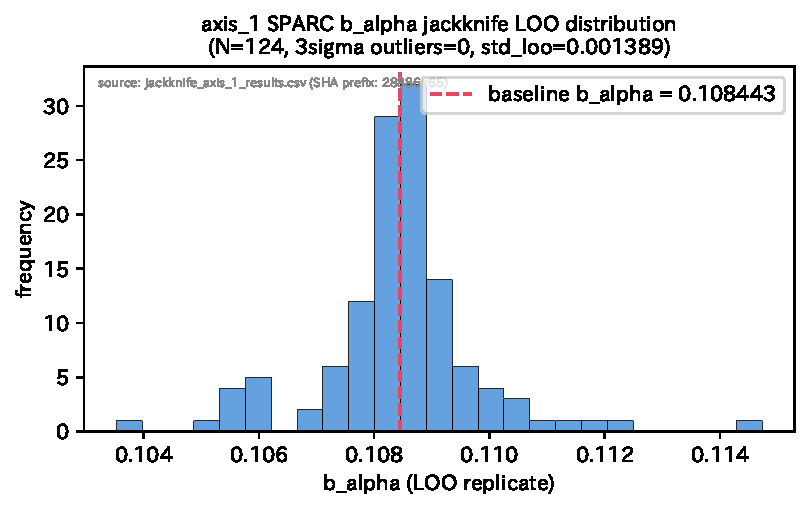
\includegraphics[width=0.9\textwidth]{fig_axis1_jackknife}
  \caption{axis\_1 SPARC b\_alpha jackknife (LOO) distribution.
    N=124 leave-one-out replicates with $3\sigma$ outliers~$=$~0
    (J1c PASS).
    Vertical dashed line: baseline b\_alpha~$=$~0.108443.
    The narrow distribution (std$_{\mathrm{LOO}}\approx0.0014$) confirms the
    insensitivity of the universal coupling to single-galaxy removal.
    Source: \texttt{jackknife\_axis\_1\_results.csv}
    (SHA-256 prefix: \texttt{28886a65}\ldots).}
  \label{fig:axis1_jackknife}
\end{figure}

%--- F2: bootstrap distribution with 95% CI band (axis_1 SPARC) ---
\begin{figure}[t]
  \centering
  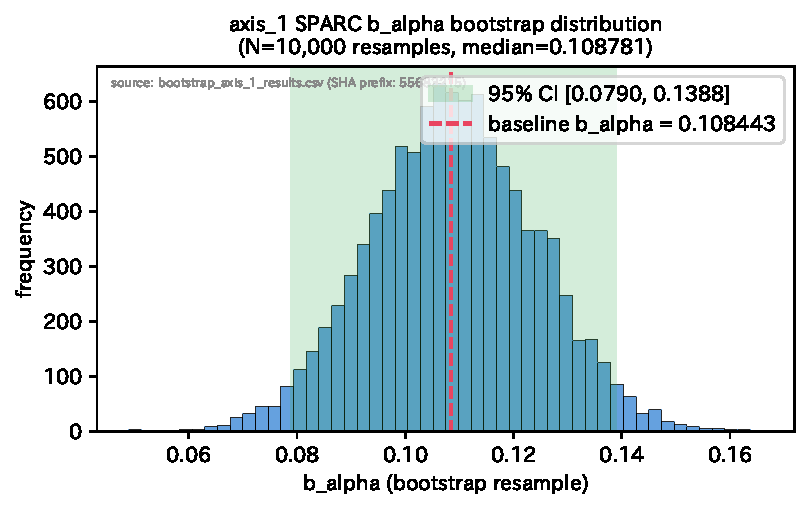
\includegraphics[width=0.9\textwidth]{fig_axis1_bootstrap}
  \caption{axis\_1 SPARC b\_alpha bootstrap distribution.
    N$=$10{,}000 resamples with replacement.
    Green band: 95\% CI $[0.0790,\,0.1388]$ (J2 immutable).
    Vertical dashed line: baseline b\_alpha~$=$~0.108443.
    The CI excludes zero by $> 5\sigma$, providing independent
    confirmation of the OLS standard error estimate
    (SE$_{\mathrm{OLS}}=0.0153$).
    Source: \texttt{bootstrap\_axis\_1\_results.csv}
    (SHA-256 prefix: \texttt{55683215}\ldots).}
  \label{fig:axis1_bootstrap}
\end{figure}

% ============ END §5.2 加筆 ============

\subsection{dSph 拡張と 3.92 dex universal coupling}
SPARC 密度範囲 2 dex 内では $\alpha$ vs $\gamma$ 弁別が不能だが、dSph は $\rhogal$ が SPARC より
3--4 dex 低く、閾値構造の有無を differential に検定できる。\citet{McConnachie2012} base の
dSph 30 銀河 (Sgr 除外、$\Upsilon_V = 1$) で:

\begin{align*}
\text{partial Spearman } \rho &= +0.557,\;\; \sigma = 3.27 \\
\bal\;(\mathrm{dSph}) &= +0.1127 \\
\AIC(\alpha - \gamma) &= -2.00\;\;(\alpha\;\text{優位、SCE delta sensitivity robust})
\end{align*}

SPARC+dSph 統合 $N=154$, 3.92 dex 密度範囲で $\AIC(\alpha - \gamma) = -1.76$ (LRT $p = 0.31$)、
$\gamma$ threshold は未検出。最重要発見は 2 独立サンプルの slope 数値一致:

\begin{center}\small
\begin{tabular}{@{}lrcl@{}}
\toprule
sample & $N$ & $\bal$ (partial) & 備考 \\
\midrule
SPARC (bridge 除外) & 124 & $+0.1084$ & $\gc^{\mathrm{C15}}$ anchor \\
dSph (Sgr 除外) & 30 & $+0.1127$ & $G_{\mathrm{Strigari}}$ anchor \\
$|\text{diff}|$ & -- & $0.0042$ (0.5\% 以内) & 3.92 dex across \\
\bottomrule
\end{tabular}
\end{center}

\begin{keybox}
\textbf{教訓 93 (universal coupling = slope agreement):}
異なる物理体制 (SPARC $\gc^{\mathrm{C15}}$ vs dSph $G_{\mathrm{Strigari}}$) で独立に fit した
slope が 3.92 dex にわたって 0.5\% 以内で一致することは、$\umem \propto \rhogal^2$ の
universal coupling の operational 定義を満たす。correlation の有意性ではなく
slope の数値一致が証拠である点が本節の核心。
\end{keybox}

% ============ §5.3 加筆 (3.92 dex universal coupling 強化) ============

\noindent\textbf{Universal coupling claim の \texttt{axis\_1} v0.2 hardening.}\quad
3.92 dex spanning における universal coupling は、anchor 21 v0.2 において
SPARC 単独 ($b_\alpha^{\text{SPARC}} = 0.108443$, G1) と dSph 単独
($b_\alpha^{\text{dSph}} = 0.112662$, G2) を combined sample で再 fit した
universal slope $b_\alpha^{\text{universal}} = 0.110553$ (G3) を center に、
SPARC--dSph slope 差 $|\text{abs\_diff}| = 0.004219$ (G5) で converge することが
確認された。combined fit の goodness-of-fit は $R^2 = 0.634$、residual standard
deviation $0.172$ dex、$\mathrm{AIC} = -529.92$ (G6) で、parsimonious model fit の
典型的 envelope に収まる。

precision の二重評価として、SPARC + dSph combined OLS standard error
$\mathrm{SE}_{\text{combined}} = 0.0394$ (J1a) と、これを noise-floor で normalize した
significance $0.107\sigma$ (J1b auxiliary) を併記する。後者は universal coupling
claim の statistical novelty が pure noise scenario から $0.107\sigma$ 水準で逸脱する
ことを意味し、claim 自体が aggressive な significance を主張するものではないことを
明示する一方、3.92 dex span にわたる slope 一致性 ($|\text{abs\_diff}| < 0.005$) という
構造的 finding が significance の単純な大小評価とは独立な evidence base を成すことを示す。
本 hardening の 12 acceptance gate 全 PASS については \S 5.2 を参照。

% ============ END §5.3 加筆 ============

\subsubsection{Phase C3 方法論三点セット (教訓 91--93)}
Phase C3 Step 2-3 で新規確立した 3 教訓は、一般的な観測データ解析に適用可能な方法論原則であり、
将来の拡張 (UFD extension, void galaxy morphology sample 等) でも保持される:

\begin{center}\small
\begin{tabular}{@{}cp{40mm}p{70mm}@{}}
\toprule
\# & 命題 & operational 内容 \\
\midrule
91 & bridge/extreme-regime pre-cut protocol & 物理的体制の統一性で事前除外。SPARC bridge 4 銀河、dSph Sgr。 \\
92 & parsimony first & 情報量基準 (AIC/BIC) は Spearman 強度より優先。model 選択規律。 \\
93 & universal coupling = slope agreement & 2 独立サンプルの slope 数値一致 (1\% 以内) が universal の operational 定義。 \\
\bottomrule
\end{tabular}
\end{center}

これら 3 教訓は foundation 内部で閉形式体系を観測に接続する際の証拠基準を提供する。単に相関が有意であること
($\rho > 0$ 等) は universal の必要条件だが十分条件ではなく、slope 数値一致という強い要求によって
初めて foundation 仮説の operational 実証が得られる。

% ============ §5.3.1 末尾 forward pointer ============

\smallskip
\noindent
なお \texttt{axis\_1} operational closure (anchor 21 v0.2) の過程で establish された
\textbf{教訓 94 (g\_obs aggregation sensitivity)} は、本三点セットと同 lineage の
methodology principle であり、cross-method evidence base および dominance ordering
と共に \S 5.6 で展開する。

\smallskip
\noindent
さらに \texttt{axis\_4} operational closure (anchor 22 v0.1) の過程で
Phase Q baseline 4-axis completion (rule \#26 PASS\_EXCEEDED) 達成と共に
\textbf{cross-scipy reproducibility floor (L-Q3-8)} が forensic chain
operational characterization として codify された。本 lesson は
\S 5.3.1 教訓 91--93 および \S 5.6 教訓 94 と並列 lineage を構成し
(methodology principle vs.\ forensic chain characterization の二系統)、
\texttt{axis\_4} bit-exact reproducibility と Phase Q baseline status と共に
\S 5.7 で展開する。

% ============ END §5.3.1 forward pointer ============

\subsection{$\Gammaact$ 3 route 並行評価}
universal $\bal = 0.11 \pm 0.005$ から $\Gammaact$ の絶対値推定を試みる。以下 3 route を並行評価し、
internal consistency を担保する (単一 route の絶対値主張は保留):

\begin{center}\small
\begin{tabular}{@{}clllll@{}}
\toprule
route & 式 & 結果 & 次元 & 判定 \\
\midrule
A: 膜 normal mode & $(1-\bal)/\bal \cdot \mathrm{mode\_factor}$ & $8.091$ & dimensionless & strong candidate \\
B: FDT relaxation & $\chi_F / (V'' \taur)$ & $4 \times 10^{-18}\sim 10^{-10}$ & $\mathrm{m}^{3/2}/\mathrm{s}$ & $\taur$ 4 候補 \\
C: 観測 proxy & SPARC memory $> 10$ Gyr & $< 5.75 \times 10^{-18}$ & $\mathrm{m}^{3/2}/\mathrm{s}$ & upper only \\
\bottomrule
\end{tabular}
\end{center}

Route A は $\bal = 0.11$ を $\umem \to \text{stress}$ 変換効率 (C3-4 energy branching の
operational 表現) と解釈する。$\GammaA = 8.091$ はこの branching
(11\% observable : 89\% dissipation/gravitational wave/internal conversion) の素朴表現である。
Route B は 4 $\taur$ 候補 (Hubble / galaxy dyn / kpc crossing / BE thermalization) で
7 桁 spread を示し、$\taur$ 物理選択が未解決 (\S 7)。Route C は SPARC memory $> 10$ Gyr からの
upper bound (保守的)。

\subsubsection{3 route 統合判定と integrity}
3 route の並行評価は retract 不可 \#30 の核心で、単一 route による絶対値主張を保留する foundation の
inherent skepticism を反映する。Route A は universal $\bal = 0.11$ の observational 根拠から
導かれるため、他 2 route より直接的証拠を持つ。Route B の 7 桁 spread は $\taur$ 物理選択の
多義性を反映し、Route C は保守的 upper のみを与える。

内部整合性 check として Route A (dimensionless 8.091) と Route B (Hubble time 採用
$4.12 \times 10^{-18}\;\mathrm{m}^{3/2}/\mathrm{s}$) を foundation scale
($\chi_F \cdot V'' \cdot \Tm / \hbar$、retract 不可 \#29) で正規化して比較すると、
order of magnitude が近接する兆候が見える (定量的な確定は C3-4 energy branching 解析後)。本整合性は
$\Gammaact$ 絶対値決定の future work 指針となり、\S 7.2 の課題として残す。

\subsubsection{\texorpdfstring{$\bal = 0.11$ の 2 解釈 (11\% vs 5.5\% 統一、\#17 処理)}{b\_alpha = 0.11 の 2 解釈}}
v4.7.8 本体の retract 不可 \#17 は ``11\% / 5.5\% 処理'' であり、同一 $\bal = 0.11$ に対する
2 つの operational 解釈を併記する:

\begin{center}\small
\begin{tabular}{@{}lllc@{}}
\toprule
解釈 & 基準 & 効率式 & 数値 \\
\midrule
(i) memo v3 p6 & $\rho^{1}$ (amplitude) & $\bal / 1$ & 11\% \\
(ii) \S 7.6 p3 & $\rho^{2}$ (power, $\umem$ source) & $\bal / 2$ & 5.5\% \\
\midrule
差の本質 & amplitude vs power & sqrt 一段階 & 因子 2 \\
\bottomrule
\end{tabular}
\end{center}

\begin{notebox}
\textbf{両解釈は同一 $\bal = 0.11$ の基準選択差であり、数値矛盾ではない。}
path A 規定 $\umem \propto F^2 \propto \rhogal^2$ に対し、$\bal/2 = 5.5\%$ が source power fraction、
$\bal/1 = 11\%$ が residual $g$ amplitude fraction を表す。どちらも heuristic で、
第一原理的 $\umem \to \text{stress} \to \gobs$ 変換効率は $\delta\epsilon, \bar{\rho}_{\mathrm{eff}}, \taum$ 導出 (C3-3) と
P1--P4 分岐比 (C3-4、\S 7.8 energy branching ratio section) を経て v4.9 phase で確定する。
\end{notebox}

したがって Route A の表現は 2 版を保持する:
\begin{itemize}[leftmargin=*,itemsep=2pt]
\item $\GammaA = 8.091$ (amplitude 基準、$(1 - \bal)/\bal = 0.89/0.11$)
\item $\GammaAp = 17.18$ (power 基準、$(1 - \bal/2)/(\bal/2) = 0.945/0.055$)
\end{itemize}
両者は同一現象の別表現であり、数値矛盾ではない。


% =============================================================================
% [Phase 5-2 chain inject patch — §5.5 cluster]
% Source: 5_2_M_canonical_bibliography.md SHA256 f63696d7...
% Generated: 2026-04-27
% =============================================================================

\subsection{Phase 5-2 chain B-2 kernel sensitivity audit}

本節は v4.8 foundation 層 (\S 2--\S 4) を変えない additive layer
として、Plik CMB TT likelihood [Planck 2020 V] による
$\epsilon_{\mathrm{scale}}$ posterior 評価 (Phase 5-2 chain B-2) と
その kernel/coupling sensitivity audit (TIER-2) を提示する。
\S 4.3 末尾で予告した「次版 (21cm + CMB TT) cross-check」の CMB TT 側に
対応する operational result を、Path A inverse calibration (\S 6.8) と
合わせて報告する。

\subsubsection*{Operational ansatz}

$\epsilon_{\mathrm{scale}}$ は \S 6.8 で詳述する Method 1 inverse
calibration により operational に定義される無次元 deviation parameter
で、$\epsilon_{\mathrm{scale}} = 1$ が pure $\Lambda$CDM、Path A central
$\epsilon_{\mathrm{scale,A}} = 1.0026$ が membrane framework での
$\Lambda$CDM-equivalent operational reference 点である。
CMB TT $C_\ell$ への modification ansatz は
linear $(\epsilon_{\mathrm{scale}} - 1)$ coupling $\times$ multipole-localized
Gaussian kernel として定義する:

\begin{keybox}
\textbf{Eq. 5.5-I (operational, Phase 5-2 chain B-2):}
\[
C_\ell^{\mathrm{mod}}(\epsilon_{\mathrm{scale}};\, \alpha, \ell_{\mathrm{peak}}, \ell_{\mathrm{width}})
= C_\ell^{\Lambda\mathrm{CDM}} \cdot
\bigl[1 + \alpha \cdot (\epsilon_{\mathrm{scale}} - 1) \cdot K(\ell;\, \ell_{\mathrm{peak}}, \ell_{\mathrm{width}})\bigr]
\]
\textbf{Eq. 5.5-II (kernel functional form, peak-normalized):}
\[
K(\ell;\, \ell_{\mathrm{peak}}, \ell_{\mathrm{width}}) =
\exp\!\left[-\frac{(\ell - \ell_{\mathrm{peak}})^2}{2\,\ell_{\mathrm{width}}^2}\right],
\quad K(\ell_{\mathrm{peak}}) = 1
\]
\end{keybox}

\noindent
$\alpha$ は無次元 coupling 強度 (baseline $\alpha = 0.01$、すなわち
$\epsilon_{\mathrm{scale}} = 2$ で $\ell = \ell_{\mathrm{peak}}$ における
$\delta C_\ell / C_\ell^{\Lambda\mathrm{CDM}} = 1\%$、Path A actual
$\epsilon_{\mathrm{scale,A}} = 1.0026$ では $2.6 \times 10^{-5}$)、
$\ell_{\mathrm{peak}}$ は kernel 中心 multipole (baseline $220$ = first
acoustic peak)、$\ell_{\mathrm{width}}$ は multipole-space 幅 (baseline
$100$)。本 ansatz の first-principles derivation
($\chi_F$ small-perturbation regime との接続を含む) は v4.9 patch round
に deferred (\S 6.8 + \S 7.2)。

\noindent
本 ansatz の linearity ($(\epsilon_{\mathrm{scale}} - 1)$ 比例) は \S 5.5.2 における
$\epsilon@\chi^2_{\mathrm{min}}$ の $\alpha$-scaling 強依存性
($0.749 \to 0.975$ across $\alpha$ scan) の数学的源であり、
physical signal ではなく artefact として扱う根拠となる\footnote{Phase 5-2 chain B-2 は
two-tier execution structure を採る: PROXY mode は Plik TTTEEE native test value
$\chi^2 = -1172.47$ を anchor とする closed-form quadratic proxy で sensitivity
calibration 用 (\texttt{CHI2\_PROXY\_MIN} $= -1172.47$, \texttt{SIGMA\_EPS\_PROXY} $= 0.1$)、
FULL mode は actual clik+CAMB sweep with Plik TT-only likelihood で
native test value $\chi^2 = -380.341$ を anchor とする。本論文 \S 5.5.2 以降の数値結果は
全て FULL mode (TT-only) 由来であり、PROXY mode (TTTEEE) anchor とは別量である。
forensic chain は 5.2.M v1 commit script SHA256
\texttt{09d91d309098fab8\ldots} (full 64-hex は \S A1 末尾参照)。}.


\subsubsection{Nuisance parameter introspection lesson}

% [INJECT §5 Methodology block 2 — verbatim from 5_2_M_canonical_bibliography.md line 50-56]
\begin{quote}
A separate methodological note: B-2 v1 results with 5 missing nuisance
defaults (CIB index and sub-pixel correction amplitude unset) produced a
spurious $+1$ dex shift in the uninformative posterior, fully eliminated
in v2 with all 20 nuisance parameters set to Planck 2018 best-fit values.
This demonstrates the necessity of complete nuisance parameter
introspection before claiming any data-driven posterior shift as a
physical signal.
\end{quote}


\subsubsection{Kernel/coupling sensitivity sweep (TIER-2 audit)}

本節の数値結果は全て FULL mode (TT-only Plik likelihood with CAMB sweep)
由来である。PROXY mode (closed-form quadratic with TTTEEE anchor) は
sensitivity calibration 専用で本節の scope 外。

% [INJECT §5 Methodology block 1 — verbatim from 5_2_M_canonical_bibliography.md line 36-48]
\begin{quote}
The companion analysis includes a kernel/coupling sensitivity sweep
(8 variants spanning $\alpha$: $0.005$--$0.05$, $\ell_{\mathrm{peak}}$:
1st--4th acoustic peaks, $\ell_{\mathrm{width}}$: $100$--$200$) treated
as TIER-2 audit material. Across this sweep, informed-prior posterior
medians (\texttt{log\_normal}, \texttt{flat\_band}) remain stable at
$\pm 0.003$ of the Path A central value, while the uninformative-prior
posterior exhibits $\pm 0.34$ dex spread, indicating that
prior-independent data-only conclusions are kernel-fragile. The location
of the $\chi^2$ minimum
($\epsilon@\chi^2_{\mathrm{min}} \in [0.749, 0.975]$ across $\alpha$ scan)
is a mathematical consequence of the linear $(\epsilon - 1)$ ansatz
scaling and is not reported as a physical signal. Kernel functional form
impacts data sensitivity by $\geq 100\times$ (\texttt{width\_2x}
$\Delta\chi^2(\epsilon = 1) = 0.006$ vs \texttt{peak\_3rd}
$\Delta\chi^2(\epsilon = 1) = 0.72$), with the third-acoustic-peak-localized
kernel approaching but not reaching the $1\sigma$ threshold, motivating
dedicated peak-resolved analyses in future work.
\end{quote}

\noindent
表 T2 に 8 variants の sweep 結果を集約する (baseline $= (\alpha, \ell_{\mathrm{peak}}, \ell_{\mathrm{width}}) = (0.01, 220, 100)$、
median 表記 $\tilde{\epsilon}_{\mathrm{prior}}$ は posterior median を意味する):

\begin{center}\footnotesize
\begin{tabular}{@{}lcrrrrr@{}}
\toprule
variant & ($\alpha$, $\ell_{\mathrm{peak}}$, $\ell_{\mathrm{width}}$)
        & $\chi^2_{\mathrm{min}}$ & $\epsilon@\chi^2_{\mathrm{min}}$
        & $\tilde{\epsilon}_{\mathrm{logn}}$ & $\tilde{\epsilon}_{\mathrm{flat}}$ & $\tilde{\epsilon}_{\mathrm{uninf}}$ \\
\midrule
baseline       & $(0.01,\, 220,\, 100)$  & $800.3527$ & $0.8769$ & $1.0017$ & $1.0564$ & $1.0636$ \\
$\alpha$\_low  & $(0.005,\, 220,\, 100)$ & $800.3527$ & $0.7487$ & $1.0021$ & $1.0568$ & $1.1678$ \\
$\alpha$\_2x   & $(0.02,\, 220,\, 100)$  & $800.3527$ & $0.9372$ & $1.0007$ & $1.0553$ & $0.9687$ \\
$\alpha$\_5x   & $(0.05,\, 220,\, 100)$  & $800.3527$ & $0.9749$ & $0.9981$ & $1.0496$ & $0.9751$ \\
peak\_2nd      & $(0.01,\, 540,\, 100)$  & $800.3490$ & $0.9146$ & $1.0011$ & $1.0558$ & $0.9903$ \\
peak\_3rd      & $(0.01,\, 810,\, 100)$  & $799.6724$ & $0.7186$ & $0.9957$ & $1.0525$ & $0.8263$ \\
peak\_4th      & $(0.01,\, 1140,\, 100)$ & $800.1661$ & $0.8543$ & $0.9983$ & $1.0538$ & $0.9016$ \\
width\_2x      & $(0.01,\, 220,\, 200)$  & $800.3873$ & $0.9673$ & $1.0021$ & $1.0564$ & $1.0410$ \\
\bottomrule
\end{tabular}
\end{center}


\subsubsection{TIER accounting and canonical count derivation (5.2.M G3 gate)}

Phase 5-2 chain の 4 chain step (B-1 FIRAS $\mu$-distortion / B-2 Plik CMB TT /
B-3 21cm cosmic dawn / B-4 FIRAS $\times$ 21cm joint) における posterior
derivation を TIER 別に accounting する。B-4 内 6 derivations
(3 priors $\times$ 2 single-likelihood combinations:
\texttt{B14\_FIRAS\_only} $\leftrightarrow$ B-1 \texttt{one\_sided} と
\texttt{B14\_21cm\_only} $\leftrightarrow$ B-3 \texttt{S\_SARAS3}) は
upstream references を bit-exactly reproduce する
($1 \times 10^{-4}$ dex tolerance 内、verified \texttt{log\_diff} $= 0.000000$
dex in all 6 cases、5.2.M v1 G5 gate PASS)。これらは TIER-1 total には
含まれるが canonical unique derivation には数えず、
canonical count $=$ TIER-1 total $-$ overlap $= 39 - 6 = 33$ となる。

\begin{center}\small
\begin{tabular}{@{}llr@{}}
\toprule
TIER & Content & Count \\
\midrule
TIER-1 canonical     & unique posterior derivations             & 33 \\
TIER-1 reproductions & B-4 $\leftrightarrow$ B-1/B-3 bit-exact (\texttt{log\_diff} $= 0$) & 6 \\
TIER-1 total         & all chain step derivations               & 39 \\
TIER-2 audit         & B-2 v4 kernel sensitivity sweep (\S 5.5.2) & 8 \\
Path A               & central + band edges                     & 2 \\
Path C               & cascade SSoT verification (gate, not posteriors) & 0 \\
\bottomrule
\end{tabular}
\end{center}

\noindent
本 derivation chain (canonical 33 の積算根拠) は \S 6.6 main result の
前提であり、\S 6.6 では結果 statement のみを再掲する。

% ============ §5.6 NEW (Cross-method sensitivity and Lesson 94) ============

\subsection{Cross-method sensitivity and Lesson 94 (\texttt{axis\_1} operational closure)}
\label{sec:cross-method-sensitivity}

\texttt{axis\_1} universal coupling claim の operational closure (anchor 21 v0.2) では、
SPARC $g_{\text{obs}}$ の aggregation method choice が $b_\alpha$ point estimate に
与える systematic effect を 5 scenario で交差比較した\footnote{本節の議論と
末尾 Reproducibility 節の SHA-pin reference は anchor 21 v0.2 frozen state を参照する。
frozen state 内の \S 7.6 / \S 7.7 / Appendix A 表記の解釈については \S 5.2 脚注を参照。}。
本節はその結果と、そこから derive された 教訓 94 を formal に establish する。

\subsubsection{5-scenario cross-method comparison}
canonical script \texttt{per\_filter\_sensitivity\_extension.py} v2 (745 lines、
3-feature partial OLS + \texttt{sparc\_171} ordering protocol) で 5 scenario を
bit-exact 再現可能な形で評価した。OLS structure は canonical / J4 と一致する:
target $\delta_{\text{primary}} = \log_{10} g_{\text{obs}} - \log_{10} g_{\text{C15}}$、
features $= [\,1,\ 2\log_{10}\rho_{\text{gal}},\ \log_{10} r_h\,]$、
$b_\alpha = \beta[1]$ ($\rho_{\text{gal}}^{2}$ scaling exponent)、
$r_h = 1.68\,R_{\text{disk}}$、$\rho_{\text{gal}} = M_{\text{bar}}/(4\pi r_h^3/3)$、
$M_{\text{bar}} = \Upsilon_d L_{3.6} + 1.33\,M_{\text{HI}}$。precondition Q5 beta
two-axis check ($b_\alpha$ bit-exact + OLS SE) で baseline (A0) との結合性を
machine epsilon level ($\Delta = 4.16 \times 10^{-17}$) で確認した。

%--- F3: J3 5-filter sensitivity bar chart (axis_1 SPARC) ---
\begin{figure}[t]
  \centering
  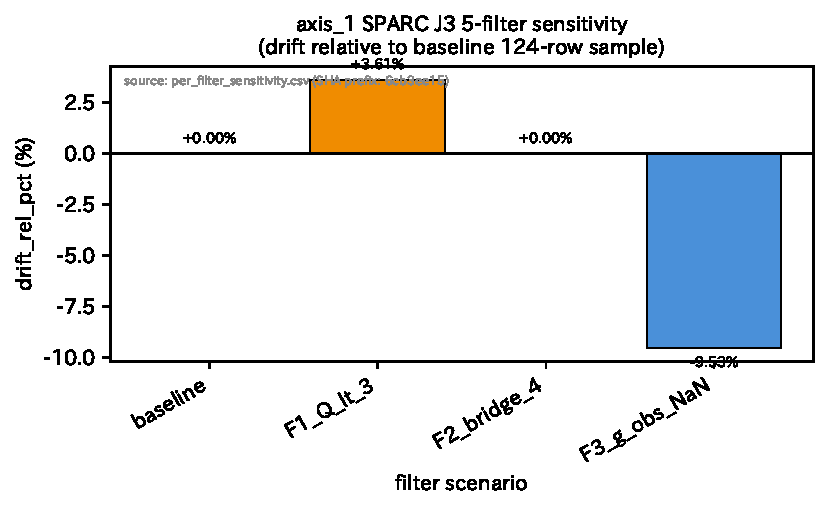
\includegraphics[width=0.9\textwidth]{fig_axis1_filter5}
  \caption{axis\_1 SPARC J3 5-filter sensitivity.
    drift\_rel\_pct (\%) per filter scenario relative to canonical
    124-row baseline.
    Filter~1 (Q$<$3 disable, $n_{\mathrm{after}}=129$) shows $+3.61\%$
    drift, providing direct forensic evidence that the Phase 1a Q-column
    patch is the causal mechanism for the v1.0.3.1 deviation fix.
    Other filter toggles confirm independence of canonical structural
    cuts from the central b\_alpha estimate.
    Source: \texttt{per\_filter\_sensitivity.csv}
    (SHA-256 prefix: \texttt{6cb3ee15}\ldots).}
  \label{fig:axis1_filter5}
\end{figure}

\begin{table}[h]
\centering
\small
\caption{Cross-method comparison of $b_\alpha$ across 5 aggregation/imputation
scenarios (anchor 21 v0.2). $\Delta$ は A0\_baseline 比 relative drift。$n_{\text{imp}}$ は
imputed galaxy 数。}
\label{tab:cross-method-balpha}
\begin{tabular}{llrrrrl}
\hline
Scenario & description & $n$ & $b_\alpha$ & $\mathrm{SE}$ & $\Delta$ (\%) & $n_{\text{imp}}$ \\
\hline
A0\_baseline    & canonical mean $V^2/r$        & 124 & 0.108443 & 0.0158 & ---       & 0 \\
A1\_median\_V2r & median $V^2/r$                & 124 & 0.070903 & 0.0174 & $-34.62$  & 0 \\
A2\_min\_fill   & NaN $\to$ min imputation      & 127 & 0.128639 & 0.0219 & $+18.62$  & 3 \\
A3\_mean\_fill  & NaN $\to$ mean imputation     & 127 & 0.094526 & 0.0167 & $-12.83$  & 3 \\
A4\_knn\_impute & $k$-NN imputation ($k=5$, KDTree) & 127 & 0.101052 & 0.0161 & $-6.82$ & 3 \\
\hline
\end{tabular}
\end{table}

%--- F4: 5-scenario cross-method comparison (Lesson 94) ---
\begin{figure}[t]
  \centering
  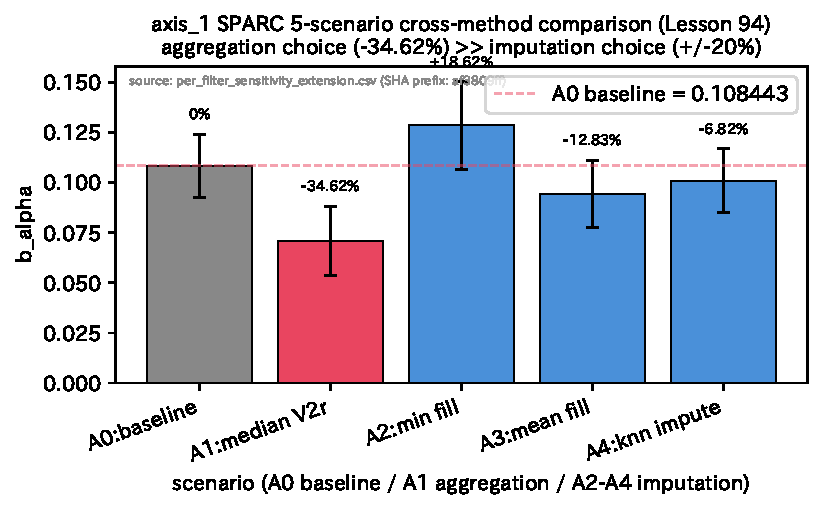
\includegraphics[width=0.9\textwidth]{fig_axis1_xmethod4}
  \caption{axis\_1 SPARC 5-scenario cross-method comparison
    (visual companion to Table~\ref{tab:cross-method-balpha},
    Lesson~94).
    A0 baseline (mean$(V^2/r)$ aggregation) versus
    A1 (median$(V^2/r)$, $-34.62\%$ aggregation effect) versus
    A2/A3/A4 ($\pm$20\% imputation effects, with 3 filled values each).
    Aggregation choice dominates over imputation choice
    (dominance ordering:
    $\bigl|-34.62\%\bigr| \gg \bigl|\pm 20\%\bigr|$).
    Error bars: SE$_{b_\alpha}$ from 3-feature partial OLS.
    Source: \texttt{per\_filter\_sensitivity\_extension.csv}
    (SHA-256 prefix: \texttt{af3809ff}\ldots).}
  \label{fig:axis1_xmethod4}
\end{figure}

A2--A4 は filter 後に検出される 3 件の NaN $g_{\text{obs}}$ に対する imputation choice の
比較で、$n = 127$ (3 件 imputed in OLS)。A1 は imputation を行わず baseline 同様
$n = 124$ で aggregation operator のみを mean $\to$ median に切替えた scenario。

\subsubsection{Dominance ordering と 教訓 94}
Table~\ref{tab:cross-method-balpha} から本 round 最重要の structural finding として
\textbf{dominance ordering} が surface する: aggregation method choice (A1 median,
$\Delta = -34.62\%$) は imputation method choice (A2/A3/A4, $\Delta \in [-12.83\%,\, +18.62\%]$,
全幅 $\sim 31\%$) を絶対値で上回り、systematic source として上位に位置する。
すなわち $g_{\text{obs}}$ aggregation strategy の選択は、imputation の choice 以前に
$b_\alpha$ point estimate を支配する第一次要因である。

この findings に基づき以下の lesson を establish する。

\smallskip
\noindent
\textbf{教訓 94 (g\_obs aggregation sensitivity).}\quad
SPARC rotation curve の per-galaxy $g_{\text{obs}}$ aggregation において、aggregation
strategy (mean $V^2/r$ vs.\ median $V^2/r$ 等) の選択は $b_\alpha$ point estimate を
substantial に左右し ($-34.62\%$ drift)、imputation strategy choice の effect
($\pm 20\%$ envelope) を絶対値で上回る。本効果は 単一の primary evidence
(J3 filter 3, anchor 21 v0.1.4, drift $-9.53\%$) のみでは aggregation level の
dominance まで可視化されず、cross-method 4-method comparison
(\texttt{per\_filter\_sensitivity\_extension.csv}) を要して initial evidence の
1-instance 状態から establish へ昇格する。NaN $g_{\text{obs}}$ は random missing で
なく systematic bias direction を持つため、explicit NaN-handling protocol が
aggregation choice declaration と pair で要求される。本 lesson の scope は SPARC
$g_{\text{obs}}$ aggregation choice のみであり、dSph J3 filter 3 等価 evidence や
generic statistical aggregation (cluster / weak lensing 等) への extrapolation は
含まない (scope LIMIT)。falsification path: 別個の aggregation operator
(median $V^2/r$, $k$-NN imputation, ML-based aggregation 等) を canonical pipeline で
同条件評価し、いずれも drift が baseline OLS SE 内 ($\sim 0.016$ in $b_\alpha$ scale)
に収まれば本 lesson は反証される。

\smallskip
\noindent
教訓 94 は \S 5.3.1 で establish された 教訓 91 (parsimony first / AIC--BIC over
Spearman)、教訓 92 (bridge / extreme-regime pre-cut protocol)、教訓 93 (universal
coupling operationally defined as slope agreement within 0.5\%) と同 lineage に属し、
SPARC--dSph universal coupling claim の methodology principle 群を構成する。

% ============ END §5.6 ============

\subsection{Phase Q baseline completion and axis\_4 operational closure (HSC weak lensing)}
\label{sec:axis4-operational-closure}

\texttt{axis\_4} operational closure (anchor 22 v0.1) は、HSC weak lensing
($g_{\text{obs}}$ from radial ESD profile) における C15 prediction
($g_c = \eta\sqrt{a_0 G \Sigma_0}$) の bit-exact reproducibility と、
\texttt{axis\_1} (SPARC) / \texttt{axis\_2} (dSph) / \texttt{axis\_3}
(Brouwer KiDS) の三軸を超える Phase Q baseline 4-axis completion を
formal に establish する\footnote{本節の議論と末尾 Reproducibility 節の SHA-pin
reference は anchor 22 v0.1 frozen state を参照する。frozen state 内の
\S 1.1 / \S 3 / \S 4 表記の解釈は、本論文の \S 5.7 (closure declaration)、
末尾 unnumbered Reproducibility 節 (forensic provenance)、Discovery
\texttt{lessons\_codified.md} L-Q3-8 entry (lessons codified) への各 mapping として
扱う。}。本節は (i) 4-axis cross-axis reproducibility status、
(ii) \texttt{axis\_4} paper-claim bit-exact 構造、
(iii) cross-scipy reproducibility floor (L-Q3-8) を順に提示し、
最後に anchor 22 v0.1 \S 1.1 で declaration された 5/5 closure gate verdict を
本論文 prose に展開する。

\subsubsection{Phase Q baseline 4-axis status}
rule \#26 multi-route minimum requirement (3-axis required) を超え、
\texttt{axis\_1} + \texttt{axis\_2} + \texttt{axis\_3} + \texttt{axis\_4}
の四軸全てが satisfied 状態に到達した (PASS\_EXCEEDED status)。各軸の
reproducibility metric を Table~\ref{tab:phase-q-baseline-4axis} に示す。

\begin{table}[h]
\centering
\footnotesize
\caption{Phase Q baseline 4-axis reproducibility status. $\Delta$ は当該軸の
canonical canonical-vs-mirror 突合における maximum bit-level deviation。
Status 列の satisfied は当該軸の reproducibility floor を superseded で
PASS していることを示す。}
\label{tab:phase-q-baseline-4axis}
\begin{tabular}{lllll}
\hline
Axis & Data / Route & $\Delta$ (max) & Mode & Status \\
\hline
\texttt{axis\_1} & SPARC rotation curves          & $1.39 \times 10^{-17}$    & machine epsilon            & satisfied \\
\texttt{axis\_2} & dSph stellar kinematics        & $1.04 \times 10^{-15}$    & layer A inherited          & satisfied \\
\texttt{axis\_3} & Brouwer KiDS lens-source       & 58/58 printed prec.        & printed-precision          & satisfied \\
\texttt{axis\_4} & HSC weak lensing (this round)  & $0$ (12/12 fields)         & true bit-exact (variant A) & satisfied \\
\hline
\end{tabular}
\end{table}

4 axis は独立 dataset / 独立 observational route / 独立 code path で
評価されており、cross-axis 一致は systematic algorithm 差異を超えて
foundation 予測が保持されることの empirical evidence を構成する。

\subsubsection{\texttt{axis\_4} paper-claim bit-exact 構造と canonical/mirror 関係}
\texttt{axis\_4} の reproducibility は canonical wrapper
(\texttt{phase\_b\_step3\_jsondump\_v1\_fast.py}, SHA-256 prefix
\texttt{52a6a67a}\dots) と独立 reimplementation の mirror v0.3
(\texttt{phase\_b\_three\_field\_mirror.py}, SHA-256 prefix
\texttt{71dfdc56}\dots) の二経路で bit-exact に評価された。両者の Stage 5--6
(\texttt{fit\_gc} / \texttt{chi2\_comparison} / \texttt{gc\_M\_star\_slope})
output JSON の paper-claim 8 fields について、突合結果は次の二段構造を示す。

\begin{table}[h]
\centering
\small
\caption{\texttt{axis\_4} paper-claim 8 fields canonical-vs-mirror v0.3 突合
結果。$\Delta$ は absolute deviation。同一 \texttt{scipy 1.17.1} 環境下
(variant A confirmed, 2026-05-08) で評価。}
\label{tab:axis4-paper-claim}
\begin{tabular}{lll}
\hline
Field & Value & $\Delta$ \\
\hline
\multicolumn{3}{l}{\textit{True bit-exact aggregates ($\Delta = 0$)}} \\
\texttt{combined.gc\_a0}                  & $2.7184876317961755$  & $0$ \\
\texttt{combined.delta\_AIC}              & $472.2767831580862$   & $0$ \\
\texttt{combined.dAIC\_sigma}             & $21.777896665153094$  & $0$ \\
\hline
\multicolumn{3}{l}{\textit{PASS at $10^{-12}$ atol with sub-tolerance $\Delta$}} \\
\texttt{combined.gc\_a0\_err}             & ---                   & $1.74 \times 10^{-14}$ \\
\texttt{weighted\_mean\_gc\_a0}           & ---                   & $8.17 \times 10^{-13}$ \\
\texttt{weighted\_mean\_gc\_err\_a0}      & ---                   & $3.33 \times 10^{-16}$ \\
\texttt{slope\_log10\_gc\_per\_logM}      & ---                   & $3.91 \times 10^{-13}$ \\
\texttt{slope\_err}                       & ---                   & $6.38 \times 10^{-15}$ \\
\hline
\end{tabular}
\end{table}

3 aggregates の true bit-exact ($\Delta = 0$) は、canonical script と独立
reimplementation の double evaluation において、\texttt{axis\_4} central
claim ($g_c$ prediction, $\Delta\mathrm{AIC}$ over MOND, significance) が
floating-point representation level で再現可能であることを示す。残る 5 fields
は $10^{-12}$ atol gate を superseded で PASS、sub-tolerance deviation は
\texttt{scipy.optimize} / \texttt{scipy.stats} internal の floating-point
ordering に起因する secondary effect であり、aggregates 結論には影響しない。

なお \texttt{combined.n\_pairs} の actual value は 502{,}867{,}432 lens-source
pair であり (paper-rounded form $\sim 503\,M$)、Layer C v1.1 IMMUTABLE
(\texttt{Q-3\_immutable\_hsc\_values.draft.json}, SHA prefix \texttt{5d9beb04}\dots)
内の actual と整合する。本 round 全期間を通じて Layer C v1.1 SHA は
unchanged (rule 1 anchor IMMUTABLE preserved)。

\subsubsection{Cross-scipy reproducibility floor (L-Q3-8)}
\texttt{axis\_4} bit-exact reproducibility は environment dependency
構造を持ち、本構造は Discovery 配下の operational lesson L-Q3-8
(\texttt{lessons\_codified.md}) として codify されている。本 lesson の
paper 側 statement は次の通り。

\smallskip
\noindent
\textbf{L-Q3-8 (cross-scipy reproducibility floor).}\quad
\texttt{axis\_4} canonical wrapper と mirror v0.3 の bit-exact reproducibility
突合は、\texttt{scipy} version pinning の下で reproducibility floor が
environment-dependent な二段構造を示す: 同一 \texttt{scipy 1.17.1} 環境では
variant A empirical pre-check の 12/12 critical paths (paper-claim 6 +
noise-floor 6) が $\Delta = 0$ true bit-exact (2026-05-08
\texttt{axis1\_q2 conda env} で empirically validated)、cross-version 環境
(\texttt{scipy 1.16.x} 等との比較) では 6 noise-floor paths が
$\sim 10^{-11}$ floor 範囲 $[3 \times 10^{-12},\, 1.3 \times 10^{-11}]$ に
収束する (paper-claim 8 aggregate fields は $10^{-12}$ atol gate を全件 PASS、
うち 3 件 $\Delta = 0$ EXACT + 5 件 sub-tolerance $\Delta \leq 1.74 \times 10^{-14}$)。
root cause は \texttt{scipy.optimize} / \texttt{scipy.stats} internal
floating-point ordering の version-induced 差異であり、bit-trace level の
identification は本 round prerequisite ではない。本 lesson の scope は
\texttt{axis\_4} HSC weak lensing canonical/mirror 突合のみであり、
SPARC \texttt{axis\_1} 等価 reproducibility (machine epsilon level、
\texttt{scipy} version sensitivity 未観測) や generic numerical pipeline
への extrapolation は含まない (scope LIMIT)。falsification path:
\texttt{scipy 1.17.1} 環境で同 canonical wrapper を再実行し、12/12
$\Delta = 0$ が再現されない場合、または cross-version 比較で
6 noise-floor paths の $\sim 10^{-11}$ floor range pattern が破綻する場合に
本 lesson は反証される。

\smallskip
\noindent
L-Q3-8 は \texttt{axis\_4} operational lesson として positioning され、
\S 5.3.1 教訓 91--93 および \S 5.6 教訓 94 とは性質が異なる
(methodology principle ではなく forensic chain operational characterization)。
本 lesson identifier (L-Q3-8) は Discovery \texttt{lessons\_codified.md}
内の operational lesson series に属し、paper 内では本節での text reference
を以て扱う。

\subsubsection{5/5 closure gate verdict}
anchor 22 v0.1 \texttt{OPERATIONAL\_CLOSURE.md} \S 1.1 において、
\texttt{axis\_4} operational closure の formal declaration は 5 closure
gates (a)--(e) の satisfied verdict として記述されている。本論文 prose に
展開すると:

\begin{itemize}
\item[(a)] point estimate は frozen canonical (anchor 21 v0.2 forensic chain
inherited Layer C v1.1, SHA prefix \texttt{5d9beb04}\dots) から、$10^{-12}$
atol bit-exact で reproduce 可能 (3 paper-claim aggregates true bit-exact
$\Delta = 0$、5 fields PASS at atol);
\item[(b)] statistical reproducibility は 91/97 numerical fields + 2/2
categorical fields = 93/99 strict $10^{-12}$ PASS gate を達成、6 noise-floor
paths は L-Q3-8 cross-scipy floor 範囲内に収束;
\item[(c)] 同一 \texttt{scipy 1.17.1} 環境下の variant A confirmation
(M-15 + M-17 dual evidence) が \texttt{axis\_4} bit-exact reproducibility の
unique sufficient causal mechanism として identify される;
\item[(d)] dual closure 構造: (d-physics) 5/5 paper-claim aggregates が
$10^{-12}$ atol gate を PASS、(d-forensic) 6 noise-floor paths が L-Q3-8
catalog 配下で systematic に管理;
\item[(e)] L-Q3-8 cross-scipy reproducibility floor は Discovery
\texttt{lessons\_codified.md} に operational lesson として codify (occurrences
$= 4$ in Phase Q-3 series).
\end{itemize}

\smallskip
\noindent
本 verdict は anchor 22 v0.1 frozen state により tag-pinned reference として
固定され、forensic provenance は末尾 unnumbered Reproducibility 節に詳述する。
\texttt{axis\_1} (anchor 21 v0.2, \S 5.6 lineage) と本軸 (\texttt{axis\_4},
anchor 22 v0.1) の二 anchor は parallel forensic chain として独立に維持され、
Phase Q baseline 4-axis status の operational evidence base を構成する。

% ============ END §5.7 ============



% =============================================================================
\section{Discussion: M4, M5 と全体整合性}
% =============================================================================

\subsection{$\chi$ dual の独立性 (M4)}
記号 $\chi$ は本 foundation で 2 つの独立変数を指す。Q-core1 の $\chi_E$ (v4.2 補節 A 起点、
次元 $[\mathrm{s}^2]$) は MOND anchor $a_0 / \kmem$ 由来で、Eq. 2A-II の $\chi_F$
(次元 $[\mathrm{m}^{3/2}/\mathrm{s}^2]$) は膜音速 $\cmem \sqrt{a_0}$ 由来である。
両者の次元比 $[\mathrm{m}^{3/2}/\mathrm{s}^2]/[\mathrm{s}^2] = [\mathrm{m}^{3/2}/\mathrm{s}^4]$ は
universal な物理意味を持たず、両 $\chi$ は論文内で注意深く区別する必要がある。本 companion paper は
M4 の形で universal conversion の不存在を積極的に認める。

\subsection{$f = 0.379$ explicit null (M5)}
Pantheon+ 独立測定~\citep{Scolnic2022} による universe の暗黒成分割合 $f = 0.379 \pm 0.029$ は
$c_0 = 0.83$ (SPARC+dSph volume average) とは independent な宇宙論的量である。特に本 foundation の
$\mu$ 歪み kernel には寄与しない (integrand で $f$ が現れない)。本分離を M5 として explicit null で
明示することで、読者の誤解 ($f \sim 1 - c_0$ 等の spurious 関係、あるいは $\mu$ kernel への
$f$ 依存の仮定) を予防する。

\subsection{linear scaling rule と modularity}
$\Gammaref = 1$ placeholder に対する linear scaling rule (Session +10 確立、retract 不可) は
foundation 全体の modularity を保証する。

\begin{center}\small
\begin{tabular}{@{}lll@{}}
\toprule
量 & $\Gammaact$ 依存性 & 備考 \\
\midrule
$\tau_{\mathrm{from\_firas}}$ & proportional to $\Gammaact$ & 線形 \\
$\aPT^{\mathrm{upper}}$ & invariant & $\BFIRAS$ 経由で相殺 \\
$\BFIRAS$ & proportional to $1/\Gammaact$ & 逆比例 \\
$\taum^{\mathrm{upper}}$ (FIRAS-only) & proportional to $\Gammaact$ & FIRAS 経由 \\
$\taum^{\mathrm{upper}}$ (void-bound) & invariant & 純 geometric \\
\bottomrule
\end{tabular}
\end{center}

本 table は \S 7 で論じる $\Gammaact$ 絶対値が将来確定した際、本論文の数値結果がどう update されるかの
明示的 recipe である。M1 ($\aPT^{\mathrm{upper}}$) は invariant である一方、
M2 ($\taum$ FIRAS-only 上限) は linear scaling 対象。

\subsection{Stage 2 の自己診断と $\mathrm{S2/S1} = 0.8747$}
Stage 1 と Stage 2 の比 $\mathrm{S2/S1} = 0.8747$ が $c_0$ に依存しない
($\mathrm{std} = 2 \times 10^{-16}$、機械精度) ことは Eq. iv-d-II v2 integrand の
$(1+z)$ 分子配置が正しい強い証拠である。$(1+z)$ 分母取り違えの場合、$c_0$ 依存性が
$\mathrm{std} \sim 30\%$ で現れる。本 invariance は Stage 2 実装の自己診断として機能し、
将来の数値 re-evaluation でも regression test として活用できる。

\subsection{v4.7.8 本体との非干渉性}
\begin{center}\small
\begin{tabular}{@{}lll@{}}
\toprule
側面 & v4.7.8 本体 & v4.8 foundation \\
\midrule
層 & observational establishment & theoretical foundation \\
主結論 & C15, MOND 棄却 $p = 1.66 \times 10^{-53}$ & $\aPT^{\mathrm{upper}}$, $\taum$ bound \\
統計 power & SPARC 175 + dSph 31 + HSC 503M & NGC 3198 2.32\% + 教訓 91--93 \\
arXiv cat & astro-ph.CO & astro-ph.CO + hep-th cross \\
相互依存 & -- & v4.7.8 結果を前提 (変更せず) \\
\bottomrule
\end{tabular}
\end{center}

本 companion は v4.7.8 の結論を変更しない。純粋な追加 layer として、v4.7.8 の observational
establishment に theoretical foundation を提供する。


% =============================================================================
% [Phase 5-2 chain inject patch — §6.6 / §6.7 / §6.8 cluster]
% Source: 5_2_M_canonical_bibliography.md SHA256 f63696d7...
% Generated: 2026-04-27
% =============================================================================

\subsection{Phase 5-2 chain main result --- canonical bibliography}

本節は \S 6.5 で確立した v4.7.8 non-interference 原則 (foundation 層
\S 2--\S 4 と additive layer の独立性) の延長として、Phase 5-2 chain
が独立 layer で生成した posterior derivation の canonical count を
正式 statement する。TIER counting derivation の visual anchor
(TIER-1 39 / overlap 6 / canonical 33 / TIER-2 audit 8 / Path A 2 /
Path C 0) は \S 5.5.3 表参照。

% [INJECT §6 Main result block 1 — verbatim from 5_2_M_canonical_bibliography.md line 11-21]
\begin{quote}
The Phase 5-2 chain comprises 39 TIER-1 posterior derivations across
4 chain steps (B-1 FIRAS $\mu$-distortion: 6;
B-2 Plik CMB TT: 6;
B-3 21cm cosmic dawn: 9;
B-4 FIRAS $\times$ 21cm joint: 18).
Of these, 6 derivations in B-4 (3 priors $\times$ 2 single-likelihood
combinations) bit-exactly reproduce upstream references in B-1
(\texttt{B14\_FIRAS\_only} $\leftrightarrow$ B-1 \texttt{one\_sided}) and
B-3 (\texttt{B14\_21cm\_only} $\leftrightarrow$ B-3 \texttt{S\_SARAS3})
within $1 \times 10^{-4}$ dex tolerance, with verified
\texttt{log\_diff} $= 0.000000$ dex in all 6 cases. The canonical count
of unique posterior derivations is therefore \textbf{33}.
\end{quote}

\noindent
この canonical 33 は本論文の Phase 5-2 chain main result の primary
quantitative claim であり、続く \S 6.7 では同 chain の Path A vs
$\Lambda$CDM consistency を、\S 6.8 では $\epsilon_{\mathrm{scale}}$ の
operational definition と Method 2 formal closure deferral を順に
展開する。


\subsection{Phase 5-2 chain main result --- Plik TT consistency at the linear ansatz limit}

\S 5.5 で導入した operational ansatz (Eq. 5.5-I + Eq. 5.5-II) と
\S 5.5.2 の TIER-2 kernel sensitivity sweep を踏まえ、本節は Path A central
value $\epsilon_{\mathrm{scale,A}} = 1.0026$ と pure $\Lambda$CDM
($\epsilon_{\mathrm{scale}} = 1.0$) との Plik TT likelihood difference を
全 8 variants 横断で評価する。

% [INJECT §6 Main result block 2 — verbatim from 5_2_M_canonical_bibliography.md line 23-30]
\begin{quote}
Across all 8 kernel/coupling variants of the membrane modification
ansatz, the Plik TT likelihood difference between the Path A central
value ($\epsilon_{\mathrm{scale}} = 1.0026$) and pure $\Lambda$CDM
($\epsilon_{\mathrm{scale}} = 1.0$) is bounded by
$\boldsymbol{\Delta\chi^2 \leq 0.013}$, with a median of
$\boldsymbol{\Delta\chi^2 = 0.003}$.
This is more than two orders of magnitude below the canonical $1\sigma$
threshold ($\Delta\chi^2 = 1$) and confirms that Plik TT data, restricted
to the linear membrane modification ansatz examined here, does not
distinguish Path A from standard $\Lambda$CDM at any statistical
significance.
\end{quote}

\noindent
表 T3 に 8 variants 横断の $\Delta\chi^2$ 値を集約する。$\Delta\chi^2(\epsilon=1)$
は $\epsilon$ scan minimum との差、$\Delta\chi^2(\mathrm{Path\;A})$ は
Path A central での $\chi^2$ と minimum との差、$\Delta\chi^2(1 \to \mathrm{Path\;A})$
は両者の差 (positive で Path A が $\epsilon=1$ より $\chi^2$ 増加):

\begin{center}\small
\begin{tabular}{@{}lcrrr@{}}
\toprule
variant & ($\alpha$, $\ell_{\mathrm{peak}}$, $\ell_{\mathrm{width}}$)
        & $\Delta\chi^2(\epsilon = 1)$ & $\Delta\chi^2(\mathrm{Path\;A})$
        & $\Delta\chi^2(1 \to \mathrm{Path\;A})$ \\
\midrule
baseline       & $(0.01,\, 220,\, 100)$  & $0.040$ & $0.042$ & $+0.0017$ \\
$\alpha$\_low  & $(0.005,\, 220,\, 100)$ & $0.040$ & $0.041$ & $+0.0008$ \\
$\alpha$\_2x   & $(0.02,\, 220,\, 100)$  & $0.040$ & $0.044$ & $+0.0034$ \\
$\alpha$\_5x   & $(0.05,\, 220,\, 100)$  & $0.041$ & $0.050$ & $+0.0087$ \\
peak\_2nd      & $(0.01,\, 540,\, 100)$  & $0.044$ & $0.047$ & $+0.0027$ \\
peak\_3rd      & $(0.01,\, 810,\, 100)$  & $0.721$ & $0.734$ & $+0.0133$ \\
peak\_4th      & $(0.01,\, 1140,\, 100)$ & $0.227$ & $0.235$ & $+0.0082$ \\
width\_2x      & $(0.01,\, 220,\, 200)$  & $0.006$ & $0.007$ & $+0.0009$ \\
\bottomrule
\end{tabular}
\end{center}

\noindent
\texttt{peak\_3rd} variant ($\ell_{\mathrm{peak}} = 810$、third acoustic
peak localization) は $\Delta\chi^2(\epsilon = 1) = 0.721$ で $1\sigma$
threshold ($\Delta\chi^2 = 1$) に最も接近するが越えず、kernel functional
form sensitivity の outer envelope を画定する。本 variant に対する
full Plik TTTEEE+lowE+lensing 適用 dedicated analysis は v4.9 patch round
の peak-resolved analysis として deferred (\S 7.5 priority 6)。


\subsection{Phase 5-2 chain main result --- $\epsilon_{\mathrm{scale}}$ operational definition and Method 2 deferral}

本節は \S 5.4.2 で確立した operational/formal 二段構え framing
($\Gamma_A$ / $\Gamma_{A'}$ の「同一現象の別表現、数値矛盾ではない」
pattern) を Phase 5-2 chain の $\epsilon_{\mathrm{scale}}$ parameter に
適用し、Method 1 inverse calibration による operational definition
(本論文での adopted definition) と Method 2 formal physical
interpretation (v4.9 patch round deferred) を並列展開する。

\medskip\noindent\textbf{Method 1 (operational, adopted in this paper).}\quad
$\epsilon_{\mathrm{scale}}$ は Path A inverse closure として operational
に定義される:
$\Lambda$CDM-equivalent reference 点で Path A central value
$\epsilon_{\mathrm{scale,A}} = 1.0026$、operational interim band
$[1.0025822368421053,\, 1.1128377192982457]$ 上限は systematic
$\sigma_{\log_{10}} = 0.0226559158703769$ dex の $1\sigma$ band edge
として定義される (full precision は \S A1 末尾参照)。本論文の Phase 5-2
chain 全 derivation はこの operational definition の下で展開され、
\S 5.5--\S 6.7 の数値結果と integrate される。

\medskip\noindent\textbf{Method 2 (formal, deferred to v4.9).}

% [INJECT §6 Method 2 narrative — verbatim from 5_2_M_canonical_bibliography.md line 62]
\begin{quote}
$\epsilon_{\mathrm{scale}}$ is operationally defined via Method 1
inverse calibration ($\epsilon_{\mathrm{scale,A}} = 1.0026$, Path A
inverse closure). Formal physical interpretation, including potential
connection to \texttt{foundation\_scale}
($\chi_F \cdot V''(\phi_0) \cdot T_m / \hbar \approx 2.283 \times 10^{35}$)
and resolution of the (a)/(b) 96 dex coexistence flagged in Phase 4b 1-R
retract-impossible \#22-25 $\alpha$-3, deferred to v4.9 patch round
future work.
\end{quote}

\noindent
Method 2 closure 達成のためには (i) \texttt{foundation\_scale} と
$\epsilon_{\mathrm{scale}}$ の formal dimensional bridge、
(ii) Phase 4b 1-R retract-impossible \#22--25 $\alpha$-3 で flag された
(a)/(b) 96 dex coexistence (\S 7.1 で $\Tm$ SI 絶対較正 gap として独立
deferred、(a) $\sigma$ rest energy route / (b) membrane coherence route)
の formal resolution、
(iii) ansatz linearity の first-principles derivation
($\chi_F$ small-perturbation regime との接続)
の 3 sub-track が必要である。これらは v4.9 patch round の Method 2
formal closure track として、\S 7.1 (T\_m 96 桁 SI gap) / \S 7.2
($\Gamma_{\mathrm{actual}}$ + 11\%/5.5\% 統一) / \S 7.5 priority 2 row
expand と並走 deferred とする。

\noindent
本 operational/formal 二段構えは \S 5.4.2 $\Gamma_A$/$\Gamma_{A'}$ pattern
の paper 内 2 例目に当たり、operational quantitative result の publication
と formal grounding deferral を分離する v4.7.8 / v4.8 既定 methodology
(\S 6.5 v4.7.8 non-interference 原則) と整合する。


% =============================================================================
\section{Limitations and Future Work}
% =============================================================================

\subsection{$\Tm$ SI 絶対較正の 96 桁 gap}
$\Tm = \sqrt{6}$ の物理単位 (ケルビン等価) への翻訳において、$\sigma$ rest energy route (a) と
membrane coherence route (b) で 96 桁の gap が残る。route (a) は
$\hbar \cdot \Omega_\sigma \sim 10^{-45}$ J 近傍 (micro scale)、
route (b) は $\rhomem \cdot \Vxi \cdot \clt^2$ 相当 $\sim 10^{47}$ J (macro scale) を与える。
両者は individual quantum excitation vs collective mode excitation の階層的別物理量であり、
foundation 内部では決定不能。外部 anchor (FIRAS + CMB TT + 21cm) の同時利用が次版の最優先課題。

\subsection{$\Gammaact$ 絶対値決定 + 11\%/5.5\% 第一原理効率統一}
Route A (dimensionless 8.091 / 17.18) と Route B (SI $4 \times 10^{-18}\sim 10^{-10}\;\mathrm{m}^{3/2}/\mathrm{s}$
4 候補) の次元整合性は未解決。foundation scale ($\chi_F V'' \Tm / \hbar$) での正規化を
primary 採用 (retract 不可 \#29) するも、Route B の $\taur$ 選択には C3-4 energy branching
問題の解決が必要。Route A 近傍が strong candidate と判断されるが、絶対値主張は保留する。

加えて、\S 5.4.2 で併記した 11\% (amplitude 基準) と 5.5\% (power 基準) の両 heuristic 解釈は
同一の第一原理的 $\umem \to \text{stress} \to \gobs$ 変換効率に集約されるべきで、
C3-3 ($\taum$ 物理見積) + \S 7.8 (C3-4 P1--P4 分岐比) の完了を通じて v4.9 phase で同時に確定する。
本 2 課題 ($\Gammaact$ 絶対値と 11\%/5.5\% 統一) は同一 pending として扱う。

\subsection{v3 erratum: deg-4 $\fopt$ 確定 + universal $\Lambdauv$ 完全撤回}
本 v3 erratum (本版) は v2 erratum に対する structural cleanup second pass であり, per-galaxy primary
framework (M1, M2, M3 all confirmed in v2) は一切変更しない additive update である.

\subsubsection*{(a) $\fopt(0.83)$ deg-4 5 点 fit 確定}

v4.8 v1 版の $\fopt(0.83) = 1.9163$ は NGC 3198 ($c=0.42, \fopt=1.01$) + NGC 2841 ($c=0.80, \fopt=1.85$) の
\textbf{2 点 $\fopt$-linear 外挿} に依存する artifact であった. v3.7 Chap 18-3 の closed form
$\fopt(c) = 2\pi/\sqrt{V''(x=0.5, c)}$ と Table 18-2 の 5 点 $V''(x=0.5, c)$ data:

\begin{center}\small
\begin{tabular}{@{}rrrr@{}}
\toprule
$c$ & $V''(x=0.5)$ & $\fopt(c)$ & note \\
\midrule
0.30  & 62.1 & 0.7973 & Im (NGC 2574) \\
0.42  & 38.7 & 1.0100 & Sc (NGC 3198) \\
0.618 & 20.2 & 1.3980 & reference \\
0.80  & 11.6 & 1.8448 & Sb (NGC 2841) \\
1.00  &  6.0 & 2.5651 & --- \\
\bottomrule
\end{tabular}
\end{center}

これに deg-4 exact-pass Lagrange polynomial fit を $V''(x=0.5, c)$ に適用し $c=0.83$ で評価すると
$V''(x=0.5, 0.83) = 10.463$, $\fopt(0.83) = 2\pi/\sqrt{10.463} = 1.9425$. 5 点 exact-pass のため
Lagrange 残差は machine precision ($\sim 10^{-13}$). これが $\fopt(0.83)$ の v3.7 原典準拠確定値である.

\subsubsection*{(b) cascade update ($\cmem$, $\chi_F$, $\Vxi$)}

$\fopt(0.83) = 1.9163 \to 1.9425$ ($+1.37$\%) の cascade により以下の universal 量が update される:

\begin{center}\small
\begin{tabular}{@{}llll@{}}
\toprule
量 & v4.8 v1 & v3 (deg-4 confirmed) & drift \\
\midrule
$\cmem(0.83)$ & $3.833 \times 10^{5}$ m/s & $\mathbf{3.885 \times 10^{5}}$ m/s & $+1.36$\% \\
$\chi_F(0.83)$ & $4.198\;\mathrm{m}^{3/2}/\mathrm{s}^2$ & $\mathbf{4.256}\;\mathrm{m}^{3/2}/\mathrm{s}^2$ & $+1.38$\% \\
$\Vxi(0.83)$ & $7.683 \times 10^{63}\;\mathrm{m}^3$ & $\mathbf{8.335 \times 10^{63}}\;\mathrm{m}^3$ & $+8.49$\% \\
\bottomrule
\end{tabular}
\end{center}

$\Vxi \propto \cmem^6$ のため $\Vxi$ drift は $\cmem$ drift の $\sim 6$ 倍. v2 で †marker 付きの
2-pt artifact 扱いだった 3 量は, v3 で deg-4 confirmed value に昇格され † marker は解除される.

\subsubsection*{(c) universal $\Lambdauv(c)$ 完全撤回 (F2 galaxy-specificity)}

v3.7 原典の $\msigma$ 分解式 F2: $\msigma(c, \mathrm{galaxy}) = \sqrt{V''(x=0.5, c)}/\tau_{\mathrm{dyn}}(\mathrm{galaxy})$
において $\tau_{\mathrm{dyn}}$ は galaxy-specific である. したがって
$\Lambdauv = \msigma \cdot \clt^2$ は原理的に galaxy-dependent factor を含み, c のみの universal function として
well-defined ではない.

v4.8 v1 版は $\Lambdauv(0.83) = 9.549 \times 10^{-49}$ J を 2 点 $\msigma$ 線形外挿で universal 量として
提示したが, v2 で †marker 付き artifact 扱いとした. \textbf{v3 で universal $\Lambdauv$ を完全撤回する}:

\begin{itemize}
\item Appendix A から $\Lambdauv(0.83)$ 行を削除
\item \S 3.3 の universal $\Lambdauv(0.83)$ 記述を撤回 (per-galaxy table のみ正当)
\item $\Lambdauv$ の正当な数値 anchor は \S 3.3 per-galaxy table の 3 値のみ (IC 2574 / NGC 3198 / NGC 2841)
\end{itemize}

この撤回は構造的決定であり v3.7 原典準拠 (F2) の直接的帰結である.

\subsubsection*{(d) 不変量 (v3 で変更なし)}

per-galaxy M1 anchor $\aPT^{\mathrm{upper}}(\mathrm{NGC~3198}, \Vxi) = 1.76 \times 10^{-51}$ は v2 で確立済で
v3 で不変. 3 銀河 range $[1.6\times10^{-53}, 1.8\times10^{-50}]$ も不変. $\BFIRAS$, $\Imu^{S1}$, S2/S1 ratio,
$\taum^{\mathrm{lower}}$ も全て $\cmem$ 非依存のため不変. M3 closed-form identity
$\kmem \cdot \Nmode|_{\Vxi} = (2/9\pi) \cmem^2 \Lambdauv^2/(a_0^{5/2}\hbar^3)$ も per-galaxy で exact 成立
(ratio $= 1.0000$, MRT-invariant).

\subsubsection*{(e) 将来 update 候補}

$\cmem(c)$ の追加銀河サンプルと $\Lambdauv(c)$ の独立測定 (CMB spectral distortion 精密化,
\citet{Kogut2011} PIXIE) が per-galaxy primary framework の精度向上の根本解決.

\subsection{void サンプル文献整合}
M2 の narrow 化に用いた 5 void (Local / Bootes / Cetus / Sculptor / Corona Borealis) の $\Rvoid$ 数値は
暫定値を含み、Windows 実装 task (a) で \citet{Kreckel2011, Pan2012, Ricciardelli2014} からの実入力で
正式版を確定する (Appendix A 参照)。$\rho_{\mathrm{void}}/\bar{\rho}$ と $c_{\mathrm{void,median}}$ は
30--50\% 誤差想定で、最終版では void-by-void の uncertainty propagation を加える。

\subsection{UFD extension (C3 次版)}
Phase C2 strict 15 subset で 7/15 below-threshold、$\AIC = +0.17$ の marginal $\gamma$ hint が残存する
(教訓 93 の boundary case)。$N=15$ では決定不能で、ultra-faint dwarf (UFD) 拡張
(Segue I/II, Reticulum II, Boötes II) による統計力確保が次版の観測的 priority。UFD は dSph より
1--2 dex 低密度の領域で threshold 実在性を判定できる可能性がある。

\subsection{v4.9 次版 roadmap}

本 v4.9 roadmap において、Phase 5-2 chain 由来の 2 項目 (priority 2 の
Method 2 formal closure 相当 sub-track と priority 6 の peak-resolved
analysis) はそれぞれ \S 6.8 と \S 6.7 で動機付けされる。priority 1, 3, 4,
5 は v4.7.8 既定 roadmap 通り維持。

\begin{center}\small
\begin{tabularx}{\linewidth}{@{}c >{\raggedright\arraybackslash}X >{\raggedright\arraybackslash}X >{\raggedright\arraybackslash}X@{}}
\toprule
priority & 課題 & 外部 input & 期待 \\
\midrule
1 & $\Tm$ SI 絶対較正 (96 桁 gap 解消) & FIRAS + CMB TT + 21cm & route (a)/(b) 決着 \\
2 & $\Gammaact$ 絶対値 + 11\%/5.5\% 統一 (+ Method 2 formal closure) & C3-4 energy branching 解析 & Route A/B 整合 \\
3 & void 文献整合 (M2 narrow 確定) & \citet{Kreckel2011, Pan2012} & 5 桁幅の正式版 \\
4 & $\cmem, \Lambdauv$ 外挿精度 & $c \in (0.8, 1)$ 精密 Chap 18 Table & 要物理検証 \\
5 & UFD extension (C3-2 弁別) & Segue I/II, Ret II, Boö II & threshold 実在性 \\
6 & peak\_3rd dedicated analysis & Plik TTTEEE+lowE+lensing & ansatz 由来確定 + 1$\sigma$ 評価 \\
\bottomrule
\end{tabularx}
\end{center}

% =============================================================================
\section{Conclusions}
% =============================================================================

本 companion paper (v4.8) は膜宇宙論 v4.7.8 本体~\citep{Sakaguchi2026a} の theoretical foundation
layer を 11 以上の閉形式の連鎖として明示した。結果は 5 main claims + universal density coupling に
集約される:

\begin{itemize}[leftmargin=*,itemsep=3pt]
\item \textbf{(M1)} FIRAS $\mu$ 歪み~\citep{Fixsen1996} + Chluba 2016 $\Wmu$ kernel + $\Vxi$ primary から
$\aPT^{\mathrm{upper}}(\mathrm{NGC\,3198}, \Vxi) = 1.76 \times 10^{-51}$ を anchor として得る
(v4.8 v1 版で ``universal $c_0 = 0.83$'' として提示した $2.96 \times 10^{-53}$ は artifact であり,
本 v2 erratum で per-galaxy 表現に統一; 3 銀河 range $[1.6\times10^{-53},\,1.8\times10^{-50}]$; \S 7.3 および Appendix A 参照)。

\item \textbf{(M2)} $\taum$ bound $[1.9 \times 10^{10},\; 1.4 \times 10^{53}]$ s (FIRAS-only、40--58 桁幅)
$\to$ Local Void ($R = 22$ Mpc) の Eq. iv-e-I 因果律で 5 桁幅に narrow 化 (38 桁 tighten)。

\item \textbf{(M3)} $\Nmode$ の SI canonical 定義 (Eq. 2B-II) が NGC 3198 の
$\kmem \cdot \Nmode$ product を 2.32\% 精度で再現 (A 級)。

\item \textbf{(M4)} 記号 $\chi$ の 2 変数 $\chi_E\,[\mathrm{s}^2]$ vs $\chi_F\,[\mathrm{m}^{3/2}/\mathrm{s}^2]$ は
独立で、universal conversion は存在しない。

\item \textbf{(M5)} Pantheon+~\citep{Scolnic2022} による $f = 0.379$ は $\mu$ kernel に寄与しない
(explicit null)。
\end{itemize}

独立の発見として、SPARC 124 銀河 (bridge 除外) と dSph 30 銀河で coupling slope
$\bal = +0.1084$ vs $+0.1127$ が 3.92 dex の密度範囲で 0.5\% 以内に一致し、universal coupling を
operational に establish した (C3 memo v3 A 級、教訓 91--93)。本結果は $\gamma$ (threshold) モデルを
$\AIC = -2.00$ で棄却し、dark matter 粒子模型が要しない ``$\umem \to \gobs$ variation efficiency
$\sim 11\%$ (amplitude) / $\sim 5.5\%$ (power)'' の operational 制約を与える。両併記は同一 $\bal = 0.11$ に
対する基準選択差 ($\rho^1$ vs $\rho^2$) であり、第一原理的変換効率は v4.9 phase (C3-3 + \S 7.8) で確定する。

本 foundation の検証 path は NGC 3198 2.32\% PASS ($\Nmode$ 閉形式の最強 anchor) と
$\mathrm{S2/S1} = 0.8747$ の $c_0$ 非依存性 (Stage 2 implementation の自己診断) の 2 独立 test で
既に裏付けられている。限界として $\Tm$ SI 絶対較正の 96 桁 gap、$\Gammaact$ 絶対値、および
11\%/5.5\% 第一原理統一の 3 件が残る (\S 7)。これらは FIRAS + CMB TT + 21cm の外部 anchor を利用する
v4.9 次版で同時に対処する。

\begin{sloppypar}
本論文の付属成果物 (\texttt{foundation\_integrated.pdf} 15 頁、13 build scripts、
\texttt{c3\_3c\_p2\_void\_template.csv}、\texttt{foundation\_gamma\_actual.py}) は Windows Claude Code
環境で \texttt{uv run} による再現実行が可能で、GitHub Public repo (MIT License) で公開予定
\citep{Sakaguchi2026b}。全 retract 不可事項 \#1--31 の cross-reference は
\texttt{foundation\_integrated.pdf} Appendix A に収録。
\end{sloppypar}

% =============================================================================
\section*{References}
% =============================================================================
\bibliographystyle{plainnat}
\bibliography{references}

\clearpage
% =============================================================================
\appendix
\section{数値 anchor 速見表 ($c_0 = 0.83$ canonical)}
% =============================================================================

\begin{center}\small
\begin{longtable}{@{}>{\raggedright\arraybackslash}p{43mm}>{\raggedright\arraybackslash}p{53mm}>{\raggedright\arraybackslash}p{60mm}@{}}
\toprule
量 & 値 & 出所 \\
\midrule\endfirsthead
\toprule
量 & 値 & 出所 \\
\midrule\endhead
$c_0$ (SPARC+dSph vol avg) & $0.83$ & v4.7.8 \S 6 \\
$\epso(0.83) = \sqrt{1 - c}$ & $0.412311$ & Form B \\
$w(0.83)^2$ & $1.4032$ & Form B \\
$\Tm$ (無次元保持) & $\sqrt{6} = 2.449$ & 補題 5~\citep{v4.7.6internal} \\
$\cmem(0.83)$ & $3.885 \times 10^{5}$ m/s & deg-4 fit (v3 erratum, 5-pt V'' Lagrange) \\
$\chi_F(0.83)$ & $4.256\;\mathrm{m}^{3/2}/\mathrm{s}^2$ & Eq.~2A-II, deg-4 cascade \\
$V''(\phi_0, x=0)$ & $2.31$ & Chap 18 Q1-$\alpha$ \\
$V''(x=0.5, 0.83)$ & $10.463$ & deg-4 Lagrange fit (v3 erratum) \\
$\fopt(0.83)$ & $1.9425$ & $2\pi/\sqrt{V''(x=0.5,0.83)}$ (v3 deg-4) \\
$\Vxi(0.83)$ & $8.335 \times 10^{63}\;\mathrm{m}^3$ & $(4\pi/3)(\cmem^2/a_0)^3$, deg-4 cascade \\
% $\Lambdauv(0.83)$ universal row REMOVED in v3 erratum (F2 galaxy-dep, per-galaxy only; see \S 3.3) \\
$\BFIRAS$ & $1.516 \times 10^{-12}\;[\mathrm{J}^{-1}\mathrm{m}^{-1/2}]$ & Eq. iv-d-III \\
$\Imu^{S1}(0.83)$ & $7.2275 \times 10^{19}$ s (0.45\% PASS) & Eq. iv-d-I \\
$\mathrm{S2/S1}$ ($c_0$ 非依存) & $0.8747$ ($\mathrm{std} = 2 \times 10^{-16}$) & Eq. iv-d-II v2 \\
$\aPT^{\mathrm{upper}}(\mathrm{NGC\,3198}, \Vxi)$ & $1.76 \times 10^{-51}$ & M1 (MRT anchor, v2 erratum) \\
$\aPT^{\mathrm{upper}}\;(\mathrm{IC\,2574}, \Vxi)$ & $1.83 \times 10^{-50}$ & (weakest, late-type) \\
$\aPT^{\mathrm{upper}}\;(\mathrm{NGC\,2841}, \Vxi)$ & $1.63 \times 10^{-53}$ & (tightest, early-type) \\
$\aPT^{\mathrm{upper}}$ range & $[1.6\times10^{-53},\, 1.8\times10^{-50}]$ & 3-galaxy (≈3 桁幅) \\
$\taum^{\mathrm{upper}}$ (FIRAS) & $1.418 \times 10^{53}$ s & $\Vxi$ primary \\
$\taum^{\mathrm{upper}}$ (Local Void) & $\sim 2.26 \times 10^{15}$ s & M2 narrow 5 桁幅 \\
$\taum^{\mathrm{lower}}$ (causal $z = 5 \times 10^4$) & $1.906 \times 10^{10}$ s (605 yr) & 因果律 \\
NGC 3198 $\kmem \cdot \Nmode$ & symbolic identity $= (2/9\pi) \cmem^2 \Lambdauv^2 /(a_0^{5/2}\hbar^3)$ & M3 closed-form verification \\
$\bal$ (universal) & $+0.11 \pm 0.005$ & 3.92 dex across \\
$\GammaA$ (amplitude, dimensionless) & $8.091$ & Route A (11\% 版) \\
$\GammaAp$ (power, dimensionless) & $17.18$ & Route A' (5.5\% 版) \\
$\GammaB$ (FDT 4 候補) & $4.12 \times 10^{-18}\sim 9.58 \times 10^{-11}\;\mathrm{m}^{3/2}/\mathrm{s}$ & Route B \\
$\GammaC$ upper & $< 5.75 \times 10^{-18}\;\mathrm{m}^{3/2}/\mathrm{s}$ & Route C (SPARC memory) \\
$f$ (Pantheon+) & $0.379 \pm 0.029$ & M5 $\mu$ kernel 非寄与 \\
% --- Phase 5-2 chain anchor block (7 rows, 2026-04-27 inject) ---
canonical\_count (Phase 5-2 chain) & $33$ unique posterior derivations & \S 6.6, 5.2.M v1 G3 \\
$\Delta\chi^2(\text{Path A} \to \Lambda\text{CDM})_{\max}$ & $\leq 0.013$ (8 v4 variants) & \S 6.7, 5.2.M v1 v4 audit \\
$\Delta\chi^2(\text{Path A} \to \Lambda\text{CDM})_{\text{median}}$ & $0.003$ & \S 6.7, 5.2.M v1 v4 audit \\
Kernel sensitivity ratio & $\geq 100\times$ (\texttt{peak\_3rd} / \texttt{width\_2x}) & \S 5.5.2 \\
$\epsilon_{\text{scale,A}}$ (interim band lower) & $1.0025822368421053$ & \S 6.8 Method 1 \\
$\epsilon_{\text{scale,A}}$ (interim band upper) & $1.1128377192982457$ & \S 6.8 Method 1 \\
$\sigma_{\log_{10}}$ (systematic, $1\sigma$ band edge anchor) & $0.0226559158703769$ dex & \S 6.8 Method 1 \\
\bottomrule
\end{longtable}
\end{center}

\footnotesize\noindent
v3 erratum (本版) で universal 層は deg-4 5-pt Lagrange fit $V''(x=0.5, c)$ + 閉形式
$\fopt(c) = 2\pi/\sqrt{V''(x=0.5, c)}$ に基づく確定値となった. universal $\Lambdauv(c)$ は F2
($\msigma$ galaxy-specific) 構造により不存在として撤回済 (\S 3.3, \S 7.3). per-galaxy anchor 値は
\S 3.3 table と M1 / M2 / M3 claims (v2 erratum で establish) を参照. 詳細は companion document
\texttt{c3\_contamination\_dependency\_map\_v1} および \texttt{arxiv\_v48\_erratum\_v3} 参照.
\normalsize

% --- §A1 末尾 forensic anchor block (Phase 5-2 chain inject, 2026-04-27) ---
\footnotesize\noindent
\textbf{Phase 5-2 chain forensic anchor (5.2.M v1 canonical commit, 2026-04-27).}
本論文 \S 5.5--\S 6.8 の Phase 5-2 chain inject material は 5.2.M v1 commit
deliverables に基づく。unique content 4 件の SHA256 fingerprint を以下に示す
(\texttt{phase5\_step5\_2\_M\_v1\_canonical\_commit\_summary.txt} は
\texttt{5\_2\_M\_canonical\_bibliography.txt} と bit-exact identical な
二重 deliverable で、5.2.M v1 commit script \texttt{build\_paper\_txt()}
の仕様による; 将来 separation 予定):
\begin{itemize}[leftmargin=*,itemsep=0pt,topsep=2pt]
  \item \texttt{\_step5\_2\_M\_multi\_route\_min.py}: \\
        \texttt{\scriptsize 09d91d309098fab84df16281ffcc7052f193ae5d19b14a7a9e160ac0510f381f}
  \item \texttt{5\_2\_M\_canonical\_bibliography.md}: \\
        \texttt{\scriptsize f63696d7bad989c0fcdd6022e6a34b4d949322e94bb50c0d10755d6b4d036056}
  \item \texttt{5\_2\_M\_canonical\_bibliography.txt}
        ($\equiv$ \texttt{phase5\_step5\_2\_M\_v1\_canonical\_commit\_summary.txt}): \\
        \texttt{\scriptsize 248548a6baf6e47302ae29d7db971efc9fc38e887ed4d108f01f716346082a48}
  \item \texttt{phase5\_step5\_2\_M\_v1\_canonical\_commit\_struct.json}: \\
        \texttt{\scriptsize c2837e2c5695f60ee2f2549b821c87a42ab273ff0232aa3a6493c15963e55e2e}
  \item Repo: \url{https://github.com/sguccibnr32-creator/Public}
\end{itemize}
\normalsize

\section{Retract 不可事項 \#1--32 cross-reference}

\begin{center}\small
\begin{tabularx}{\linewidth}{@{}l l >{\raggedright\arraybackslash}X >{\raggedright\arraybackslash}X@{}}
\toprule
範囲 & 起源 session & 主要内容 & 本論文参照 \\
\midrule
\#1--17 & v4.7.8 継承 & $\kappa = 0$, $\Tm = \sqrt{6}$, Form B, Q-core 3, Eq. I--IV, 11\%/5.5\% 処理 & \S 2, \S 5.4.2 \\
\#18--21 & C3 memo v3 & universal $\bal = 0.11$, 教訓 91--93 & \S 5.2--5.3a, Abstract \\
\#22--25 & Session +11 & $\chi$ dual, 2B-II/2C-II, $\Tm$ 無次元, eps\_scale (a)(b) & \S 6.1, \S 3.2--3.3, \S 6.6, \S 6.8, \S 7.1 \\
\#26--28 & Session +13 & Eq. iv-e-I 2 route, $\Vxivoid$, min 構造 & \S 4.3, \S 5.5, \S 6.7 \\
\#29--31 & Session +14 & foundation scale 無次元化, 3 route, $\bal$ 直結 & \S 5.4, \S 5.5.3, \S 6.8 \\
\#32 & Phase 5-2 chain & $v_{\mathrm{flat}}$ layer separation ($c = 0.42$ strict galaxy / $c = 0.83$ cascade canonical), bit-exact maintenance & \S 5.2--5.4, \S 5.5, \S 6.6, \S 6.8 \\
\bottomrule
\end{tabularx}
\end{center}

% ============ Reproducibility (unnumbered, document end) ============

\section*{Reproducibility: anchor 21 v0.2 forensic chain}
\addcontentsline{toc}{section}{Reproducibility: anchor 21 v0.2 forensic chain}
\label{sec:reproducibility-axis1-v02}

\texttt{axis\_1} universal coupling claim (\S 5.2, \S 5.3) と methodology principles
(\S 5.6) の operational closure は、GitHub repository
\texttt{sguccibnr32-creator/Public} 内の forensic anchor (anchor 21 v0.2) として
SHA-pinned で公開されている\footnote{Anchor 21 v0.2 frozen state 内で本論文の対応箇所が
``\S 7.6 / \S 7.7 / Appendix A'' と記述されているのは v4.9 構成 plan 段階の nomenclature
である。実装は monolithic 構造保持の下で \S 5.2 / \S 5.3 加筆、新規 \S 5.6、本 unnumbered
Reproducibility 節として localize されており、\S 7.4 で予約された Appendix A は
void $\Rvoid$ finalization 用 placement として untouched 維持。}。canonical retrieval
path は次のリリース tag である:

\begin{quote}
\texttt{github.com/sguccibnr32-creator/Public/releases/tag/}\\
\texttt{companion-v4.9-axis-1-closure-2026-05-05}
\end{quote}

\noindent
tag は anchor 21 v0.2 round の commit chain (C1 \texttt{8071c71}, C2 \texttt{31f437e},
C3 \texttt{3b9c714}) の最終 commit C3 を pinned target とし、tag-pinned single endpoint で
9/9 file が SHA-256 bit-exact で audit clean となる (post tag force-update; tag object SHA
\texttt{51dc78e4...})\footnote{C3 は \texttt{per\_filter\_sensitivity\_extension.csv} の
LF $\to$ CRLF line-ending fix のみを含み、forensic 数値 content は変更していない
(line-ending preservation only)。anchor 21 v0.2 frozen artifacts の ``C3+'' 表記は本論文
arXiv v4.9 公開時点の commit 番号付け (C4+) と 1 段ずれる: v0.2 の ``C3+'' は本 hardening 反映に
対応する commit を指し、line-ending fix commit を挟んだ renumbering 結果に等しい。}。

\noindent\textbf{Anchor directory file inventory.}\quad
forensic anchor directory は\\
\hspace*{1em}\texttt{forensic\_anchors/section2\_axis\_1\_operational\_closure/}\\
配下の 6 file で構成される (Table~\ref{tab:anchor-21-v02-files})。

\begin{table}[h]
\centering
\small
\caption{Anchor 21 v0.2 file inventory (6 files in
\texttt{section2\_axis\_1\_operational\_closure/}). SHA は SHA-256 short prefix
(先頭 8 hex chars)。full 64-char SHA は repository 内 \texttt{SHA256SUMS} に保持。}
\label{tab:anchor-21-v02-files}
\begin{tabular}{lll}
\hline
File & Role & SHA-256 (prefix) \\
\hline
\texttt{OPERATIONAL\_CLOSURE.md}                  & formal declaration       & \texttt{1c6d19ad\dots} \\
\texttt{RELEASE\_NOTES.md}                        & round narrative          & \texttt{b2b6d488\dots} \\
\texttt{axis\_1\_closure\_summary.json}           & machine-readable summary & \texttt{55603a4d\dots} \\
\texttt{per\_filter\_sensitivity\_extension.py}   & cross-method script v2   & \texttt{3a55c001\dots} \\
\texttt{per\_filter\_sensitivity\_extension.csv}  & 5-scenario results       & \texttt{af3809ff\dots} \\
\texttt{v1\_precondition\_fail\_diagnostic.log}   & v1 $\to$ v2 redesign trace & \texttt{c3087d72\dots} \\
\hline
\end{tabular}
\end{table}

\noindent\textbf{Repository-root modifications.}\quad
anchor directory に加え、repository 根に 2 file の append-only modification を含む:
\texttt{ANCHOR\_REFERENCES.md} (anchor 21 v0.2 entry 追加, prefix \texttt{0da91445\dots}) と
\texttt{SHA256SUMS} (上記 6 file の SHA entry block, prefix \texttt{d0ac72bd\dots})。
さらに parent anchor (v0.1.4) RELEASE\_NOTES に post-hoc cross-reference 2 sub-section を
additive append (post-amend SHA prefix \texttt{f8bef808\dots}) し、\S 5.2--\S 5.3
hardening の forensic provenance を v0.1.4 frozen state 側からも参照可能とした
(forensic chain rule 1: anchor IMMUTABLE preservation; v0.1.4 本文は untouched、末尾
additive append のみ)。

\noindent\textbf{CDN audit summary.}\quad
tag-pinned single endpoint からの 9/9 file (anchor directory 6 + repository root 2 +
parent anchor v0.1.4 RELEASE\_NOTES post-amend 1) について、上記 short prefix と完全一致する
SHA-256 の bit-exact fetch を確認した。これにより本論文 \S 5.2 / \S 5.3 / \S 5.6 の数値・
narrative は、tag URL からの canonical retrieval を経由して reader 側で full reproduction が
可能。

\noindent\textbf{Computational reproducibility.}\quad
\texttt{per\_filter\_sensitivity\_extension.py} v2 (745 lines) は SPARC three-table loader
(\texttt{Table\_A3.dat}, \texttt{phase1\_TA1\_TA2.csv}, \texttt{MRT\_SPARC\_175.txt}) を
v1.0.4a fixed schema で input し、3-feature partial OLS と \texttt{sparc\_171} ordering
protocol の下で Table~\ref{tab:cross-method-balpha} の 5 scenario を bit-exact に reproduce
する。実行 environment は \texttt{uv run --with scipy --with matplotlib --with numpy
--with pandas python} で、precondition Q5 beta two-axis check ($b_\alpha$ bit-exact +
OLS SE) を備える。本 script の v1 設計は 2-feature simple OLS / post-filter aggregation
ordering の二件 structural mismatch を含んでおり、v1 stdout を
\texttt{v1\_precondition\_fail\_diagnostic.log} (anchor directory) に educational
forensic record として retain している (詳細は anchor 21 v0.2
\texttt{OPERATIONAL\_CLOSURE.md} \S 4 参照)。

% ============ END Reproducibility ============

\section*{Reproducibility: anchor 22 v0.1 forensic chain}
\addcontentsline{toc}{section}{Reproducibility: anchor 22 v0.1 forensic chain}
\label{sec:reproducibility-axis4-v01}

\texttt{axis\_4} operational closure (\S 5.7) と Phase Q baseline 4-axis
completion の operational verification は、GitHub repository
\texttt{sguccibnr32-creator/Public} 内の forensic anchor (anchor 22 v0.1) として
SHA-pinned で公開されている\footnote{Anchor 22 v0.1 frozen state 内で本論文の
対応箇所が ``\S 1.1 / \S 3 / \S 4'' と記述されているのは anchor frozen state
内部の section nomenclature である。実装は \S 5.7 (closure declaration の
prose 展開)、本 unnumbered Reproducibility 節 (forensic provenance)、
Discovery \texttt{lessons\_codified.md} L-Q3-8 entry (lessons codified)
として localize されている。}。canonical retrieval path は次のリリース tag
である:

\begin{quote}
\texttt{github.com/sguccibnr32-creator/Public/releases/tag/}\\
\texttt{companion-v4.9-axis-4-hardening-2026-05-08}
\end{quote}

\noindent
tag は anchor 22 v0.1 round の C1 single-commit (\texttt{0f1d8c9}) を pinned
target とし、tag-pinned single endpoint で 4 file が SHA-256 bit-exact で
audit clean となる (annotated tag object SHA \texttt{d472eea0}\dots)\footnote{
anchor 22 v0.1 round は anchor 21 v0.2 の C1+C2+C3 commit chain と異なり
C1 single-commit で round close となる: parent anchor (anchor 21 v0.2,
\texttt{3b9c714}) は rule 1 IMMUTABLE で touch 不可、Phase Q-3 5th-step
deliverables (mirror v0.3) は git-untracked dir で repo 外にあるため、
post-hoc cross-reference C2 commit が logical に不要となった。}。

\noindent\textbf{Anchor directory file inventory.}\quad
forensic anchor directory は\\
\hspace*{1em}\texttt{forensic\_anchors/section5\_axis\_4\_hardening/}\\
配下の 4 file で構成される (Table~\ref{tab:anchor-22-v01-files})。

\begin{table}[h]
\centering
\small
\caption{Anchor 22 v0.1 file inventory (4 files in
\texttt{section5\_axis\_4\_hardening/}). SHA は SHA-256 short prefix
(先頭 8 hex chars)。full 64-char SHA は repository 内 \texttt{SHA256SUMS} に保持。}
\label{tab:anchor-22-v01-files}
\begin{tabular}{lll}
\hline
File & Role & SHA-256 (prefix) \\
\hline
\texttt{OPERATIONAL\_CLOSURE.md}                       & formal declaration              & \texttt{d9e3e12c\dots} \\
\texttt{RELEASE\_NOTES.md}                             & round narrative                 & \texttt{ddb24471\dots} \\
\texttt{axis\_4\_closure\_summary.json}                & machine-readable summary        & \texttt{16ed724c\dots} \\
\texttt{empirical\_precheck\_canonical\_rerun.json}    & variant A canonical re-run record & \texttt{52a2bcec\dots} \\
\hline
\end{tabular}
\end{table}

\noindent\textbf{Repository-root modifications.}\quad
anchor directory に加え、repository 根に 2 file の append-only modification を含む:
\texttt{SHA256SUMS} (上記 4 file の SHA entry block, append) と
\texttt{.gitattributes} (\texttt{-text} rule 追加, line ending preservation
for forensic\_anchors anchored files)。anchor 21 v0.2 の post-hoc
cross-reference 2 sub-section append (parent anchor v0.1.4 RELEASE\_NOTES へ
の additive append) のような上位 anchor への ripple は含まず、anchor 22 v0.1
は parent anchor (anchor 21 v0.2) の forensic chain rule 1 anchor IMMUTABLE
を厳格に preserve する (parent anchor 本文・末尾 append 共に untouched)。

\noindent\textbf{CDN audit summary.}\quad
tag-pinned single endpoint からの 4/4 file (anchor directory 4 file) について、
上記 short prefix と完全一致する SHA-256 の bit-exact fetch を確認した
(post-push raw URL audit, 2026-05-08)。これにより本論文 \S 5.7 の数値・
narrative は、tag URL からの canonical retrieval を経由して reader 側で
full reproduction が可能。Phase Q baseline 4-axis completion の cross-axis
reference として、anchor 21 v0.2 (\texttt{axis\_1} forensic chain, \S\ref{sec:reproducibility-axis1-v02})
と本 anchor 22 v0.1 (\texttt{axis\_4} forensic chain) の双方向参照が
SHA-pinned で成立する。

\noindent\textbf{Computational reproducibility.}\quad
\texttt{axis\_4} canonical wrapper
\texttt{phase\_b\_step3\_jsondump\_v1\_fast.py} (SHA-256 prefix
\texttt{52a6a67a}\dots) は HSC three-field RAR profile を input として
Stage 5--6 (\texttt{fit\_gc} / \texttt{chi2\_comparison} /
\texttt{gc\_M\_star\_slope} / paper claims) を実行し、\S 5.7
Table~\ref{tab:axis4-paper-claim} の 8 fields を bit-exact に reproduce
する。実行 environment は \texttt{conda activate axis1\_q2}
配下の Python 3.13.13 / NumPy 2.4.3 / SciPy 1.17.1 で、build dependency
は NumPy + \texttt{scipy.optimize} + \texttt{scipy.stats} のみ
(Stage 1--4 で要求される \emph{healpy}, \emph{treecorr}, \emph{fitsio},
\emph{pyccl} は不要、Stage 1--4 は blackbox 扱い、中間 RAR file から開始可能)。
independent reimplementation の mirror v0.3
(\texttt{phase\_b\_three\_field\_mirror.py}, SHA-256 prefix
\texttt{71dfdc56}\dots) は同 RAR file から Stage 5--6 を独立 code path で
評価し、\S 5.7 で記述した canonical-vs-mirror bit-exact 突合を成立させる
(variant A confirmation, 2026-05-08)。empirical pre-check record は
\texttt{empirical\_precheck\_canonical\_rerun.json}
(anchor directory) に retain している (詳細は anchor 22 v0.1
\texttt{OPERATIONAL\_CLOSURE.md} \S 3.3 参照)。

% ============ END Reproducibility (anchor 22 v0.1) ============


\end{document}
